%  \pdfoutput=1
\documentclass[10pt,journal,compsoc]{IEEEtran}
%\documentclass[10pt,journal,compsoc]{IEEEtran}
%\IEEEoverridecommandlockouts
%\settopmatter{printacmref=false} % Removes citation information below abstract
%\renewcommand\footnotetextcopyrightpermission[1]{} % removes footnote with conference information in first column
%\pagestyle{plain} % removes running headers
%\documentclass[sigconf,screen]{acmart}
\usepackage{dblfloatfix}
%\usepackage{cite} 
\usepackage{balance}
\usepackage{alltt}
\usepackage{pifont}% http://ctan.org/pkg/pifont

%\setcounter{tocdepth}{3}
%\usepackage{cite}
\usepackage{graphicx}
\usepackage{colortbl}
%\usepackage{arydshln}
%\usepackage{libertine}
%\usepackage{times}
\usepackage[dvipsnames]{xcolor}
\usepackage{rotating}
\usepackage{makecell}
\usepackage{tabularx}
\usepackage{booktabs}
\usepackage{wrapfig}
\usepackage{tikz}
\usetikzlibrary{angles}
%\usepackage{tabu}
\usepackage{multirow}
\usepackage{hyperref}
\usepackage{framed}
\usepackage[framemethod=tikz]{mdframed}
\usetikzlibrary{shadows}
\usepackage{enumitem}
\usepackage{graphics}
\usepackage[para,online,flushleft]{threeparttable}
\newcommand*\rot{\multicolumn{1}{R{30}{1.3em}}}
\setlist[description]{leftmargin=1cm}

\usepackage{pgfplots}
\usetikzlibrary{patterns}
\usetikzlibrary{arrows}
\usetikzlibrary {positioning}
\usepackage{enumitem}
\setlist[itemize]{leftmargin=*}
\setlist[enumerate]{leftmargin=*}
\usepackage{makecell}
\usepackage[linesnumbered,ruled,vlined]{algorithm2e}
\setlist{nolistsep} 

\SetKwProg{Fn}{Function}{}{}

\setlist[1]{itemsep=0pt}


\newmdenv[
tikzsetting= {fill=gray!10},
linewidth=1pt,
roundcorner=2pt,
shadow=false
]{myshadowbox}
%\usepackage[framed]{ntheorem}

\newenvironment{result}[2]
{\begin{myshadowbox}\textbf{\textit{\underline{Lesson#1:}}} #2}{
\end{myshadowbox}}
\newcolumntype{P}[1]{>{\centering\arraybackslash}p{#1}}


%        heoremclass{Lesson}
%        heoremstyle{break}

%\makeatletter
%\let        h@plain\relax
%\makeatother

\hypersetup{
    linkcolor=blue,
    filecolor=magenta,      
    urlcolor=cyan,
}
\newcommand{\tikzhighlightanchor}[1]{\ensuremath{\vcenter{\hbox{\tikz[remember picture, overlay]{\coordinate (#1 highlight \arabic{highlight});}}}}}

\newcommand{\bi}{\begin{itemize}[leftmargin=0.4cm]}
\newcommand{\ei}{\end{itemize}}
\newcommand{\be}{\begin{enumerate}[leftmargin=0.4cm]}
\newcommand{\ee}{\end{enumerate}}
\newcommand{\fig}[1]{Figure~\ref{fig:#1}}

\newcommand{\tbl}[1]{Table~\ref{tbl:#1}}
\newcommand{\eq}[1]{Equation~\ref{eq:#1}}
\newcommand{\tion}[1]{\S\ref{tion:#1}}

\usepackage{url}
%\newcommand{\keywords}[1]{\par\addvspace\baselineskip \noindent\keywordname\enspace\ignorespaces#1}
%%% graph
\newcommand{\crule}[3][darkgray]{\textcolor{#1}{\rule{#2}{#3}}}

\tikzstyle{thmbox} = [rectangle, rounded corners, draw=black, fill=gray!10]
\newcommand\thmbox[1]{%
    \noindent\begin{tikzpicture}%
    \node [thmbox] (box){%
        \begin{minipage}{.94\textwidth}%
        \vspace{-0.1cm}#1\vspace{-0.1cm}%
        \end{minipage}%
    };%
    \end{tikzpicture}}

\usepackage[tikz]{bclogo}
\newenvironment{RQ}[1]%
{\noindent\begin{minipage}[c]{\linewidth}%
\begin{bclogo}[couleur=gray!25,%
                arrondi=0.1,% 
                logo=\bctrombone,%
                ombre=true]{{\normalsize ~#1}}}%
{\end{bclogo}\end{minipage}\vspace{2mm}}



%\let        heoremframecommand        hmbox
%\newshadedtheorem{lesson}{Result}
%\newshadedtheorem{lesson1}{Result}
 
\newcommand{\quartex}[4]{
\begin{picture}(25,6)%1
    {
        \color{black}
        \put(#3,3)
        {\circle*{4}}
        \put(#1,3)
        {\line(1,0){#2}}
    }
\end{picture}
}

\usepackage{listings}
\lstset{
  basicstyle=\ttfamily,
  mathescape
}

\ifCLASSOPTIONcompsoc
  % The IEEE Computer Society needs nocompress option
  % requires cite.sty v4.0 or later (November 2003)
  \usepackage[nocompress]{cite}
\else
  % normal IEEE
  \usepackage{cite}
\fi

\ifCLASSINFOpdf
  % \usepackage[pdftex]{graphicx}
  % declare the path(s) where your graphic files are
  % \graphicspath{{../pdf/}{../jpeg/}}
  % and their extensions so you won't have to specify these with
  % every instance of \includegraphics
  % \DeclareGraphicsExtensions{.pdf,.jpeg,.png}
\else
  % or other class option (dvipsone, dvipdf, if not using dvips). graphicx
  % will default to the driver specified in the system graphics.cfg if no
  % driver is specified.
  % \usepackage[dvips]{graphicx}
  % declare the path(s) where your graphic files are
  % \graphicspath{{../eps/}}
  % and their extensions so you won't have to specify these with
  % every instance of \includegraphics
  % \DeclareGraphicsExtensions{.eps}
\fi



\newcommand\MYhyperrefoptions{bookmarks=true,bookmarksnumbered=true,
pdfpagemode={UseOutlines},plainpages=false,pdfpagelabels=true,
colorlinks=true,linkcolor={black},citecolor={black},urlcolor={black},
pdftitle={Bare Demo of IEEEtran.cls for Computer Society Journals},%<!CHANGE!
pdfsubject={Typesetting},%<!CHANGE!
pdfauthor={Michael D. Shell},%<!CHANGE!
pdfkeywords={Computer Society, IEEEtran, journal, LaTeX, paper,
             template}}%<^!CHANGE!

\hyphenation{op-tical net-works semi-conduc-tor}

\begin{document}


\title{Enhanced  Labeling of Issue Reports (with  $F^3T$)}
 
 
%\author{\IEEEauthorblockN{1\textsuperscript{st} Blinded for review}
%}

\author{Huy Tu, Tim Menzies~\IEEEmembership{IEEE~Fellow}
\thanks{Both authors are with
Computer Science, NC State, Raleigh, USA, hqtu@ncsu.edu,  timm@ieee.org}}
% \numberofauthors{3}

%\email{hqtu@ncsu.edu} 
% \affiliation{ 
%       \institution{North Carolina State University}
%       \city{Raleigh} 
%       \state{NC}
%       \country{USA}
%       \postcode{27606}
% }

\IEEEtitleabstractindextext{%
\begin{abstract}
Standard automatic methods for recognizing
problematic code can be  greatly improved  via the
incremental application of
 human+artificial expertise.
 In this approach,  call $F^3T$,  AI tools explore  software to find commits
 that they guess is most problematic.  Humans the apply their expertise to  check that guess
 (perhaps resulting in the AI
updating the  support vectors within their SVM learner).
We recommend this human+AI partnership, for several reasons.
When a new domain is encountered, $F^3T$ can  learn better ways to label which comments
refer to real problems.
Further, 
in studies with 9 open source software projects,
$F^3T$'s incremental application of human+artificial  intelligence
is at least an order of magnitude cheaper to use  than existing methods.
Lastly,   $F^3T$ is  very effective. For the data sets explored here, when compared to standard methods, 
$F^3T$  improved 
$P_{opt}(20)$ and G-scores performance by 26\% and 48\%  on median value.

% A first and vital step for many tasks of software analytics is establishing the ``ground truths'' labels. For defect prediction, identifying ``buggy'' commits is done automatically by keywords labeling as standard practices and can be improved via the incremental application of human and artificial expertise.  In our proposed $F^3T$ system, constructing the ground truths is done from a large code base via exploring the textual content of the commits to determine which changes are most likely to link to the ``buggy'' commits. Then humans apply their deep knowledge to review that guess, then the Artificial Intelligence (AI, the support vectors within a SVM learner) can update to suggest more informative in the future guesses. This human+AI partnership can be a better method for retrieving the ground truths for a specialized domain (computational science softwares, test case prioritization, identification and localization of technical-debts, defects, and bad smells) where software development is essential. In our study, $F^3T$'s incremental labeling application of human+AI provides more quality data while 12.5 times faster than existing methods.

% Data retrieval comes prediction tasks, $F^3T$'s data mining method is  highly effective with simple rule learners (4 rules with access to the labels generated via previous step) significantly out-perform complex state-of-the-art methods. 

% For the nine computational science projects explored here for defect identification and prediction on commit-level (i.e. predicting defects when the commit is made), when compared to standard systems, the proposed $F^3T$ system improved median G-scores and $P_{opt}(20)$ values by up to 48\% and 26\% respectively.



%which is borrowed from systematic literature review

%maybe something about G-score, hmmmm

\end{abstract}
 
\begin{IEEEkeywords}
Software Analytics, Human-in-the-loop AI, FFTs,  Defect prediction
\end{IEEEkeywords}}

 

\maketitle

\IEEEdisplaynontitleabstractindextext
\IEEEpeerreviewmaketitle


\ifCLASSOPTIONcompsoc
\IEEEraisesectionheading{\section{Introduction}\label{sec:introduction}}
\else
\section{Introduction}
\fi
% One of the dreams of industrial analytics is that
% new conclusions can be quickly
% obtained from new data just by throwing 
% the data at an automatic  data miner. In practice, there are many challenges before that dream can be realized.
% For example,  engineering judgment must be applied to:
% \be
% \item Categorize bug reports as ``buggy'' or not.
% \item Determine what code changes were implicated
% in a bug report;
% \item Describe code as a set of features;
% \item Cluster data prior to learning;
% \item Tune algorithms that manage class imbalance;
% \item Decide which data miners to apply;
% \item Select the control parameters for the data miners; e.g. how many trees for a random forest;
% \ee
% Note that in the above sequence
% Much recent work has explored the first five
% items. For example, Ghotra et al.  assessed how well dozens
% of data miners perform for data mining~\cite{ghotra15}.
% Applying that engineering judgment can be 
%  complex and potentially time consuming. Hence,
%  much recent
% research has focused on how to automate the above five
% tasks. Many papers 

% Much recemt
% imbalance tools These engineering decisions it has been shown that use the default tunings can lead to sub-optimal results. 

% the behavior of many data miners is
% controlled by certain tuning parameters. 


% Using software analytics takes at least four steps
% to predict   that code is buggy.
% Firstly,
%  the issues  that report software bugs must
%  be {\em labelled}.  
% Secondly, metrics  must be collected to summarize
% the code.
% Thirdly, the code changes that preceded that issue report
% must be implicated. Lastly, some classifier
% must learn to differentiate between the implicated and
% non-implicated code (using the metrics). 

% Much recent research has explored
% steps 2,3,4~\cite{} but scant attention has been given to initial labeling step. 
% In this paper, we report ways to significantly
% improve the issue labeling algorithm of step1. This new method incorporates a novel
% human-in-the-loop process in whcuh 

% The usual methods 
% Vasilescu~\cite{Vasilescu18} reports 


%A recent keynote at FSE'18~\cite{meijer18} offered a vision of ``Software 2.0'' where software is mostly written automatically by AI systems applying formal methods to rigorously defined primitives. For {\em writing} software, this does sound appealing for reducing cost and increasing the quality of released code. However, after the {\em creation} of versions of software comes the {\em maintenance} which requires human participation.  For example, once the software is released and utilized by some people, then the number of resulting issue reports can become very large.
 \IEEEPARstart{A}{} vital   first step for many software analytics tasks
is to {\em label} which  programmer commits introduce the bugs.
Such labels are required to establish the ``ground truth''
needed to train existing methods (or certify new ones).
% for tasks  
% like
% recognizing vulnerable software~\cite{yu18v}l
% identifying bad smells~\cite{KRISHNA201753}; predicting 
% defects~\cite{menzies07dp}; prioritizing test cases~\cite{zhu2018test};
% or finding
% technical debt~\cite{huang2018identifying}. 
 

% This paper shows that one widely-used labeling method  is {\em not} general.
% Specifically, {\em using  keywords to identify  ``worrying'' issue messages}
%  fails very badly when applied to different kinds of software. 
%  Much better identification can be achieved with    $F^3T$,
%  a novel combination of human+artificial intelligence.  
 
   
  
To obtain the dependent variable (i.e. bugs labels), ``worrying'' commits that indicates bug-fixing activities will be identified and utilized to trace down the buggy commits (before being fixed by ``worrying'' commits). 
Standard 
  practice~\cite{commitguru, Kim08changes,catolino17_jitmobile,nayrolles18_clever,mockus00changeskeys,kamei12_jit,hindle08_largecommits} is to 
  overlap the commit messages to keywords like  Table~\ref{tab:words}. 
  Vasilescu et al. \cite{Vasilescu15github,Vasilescu18z}  notes that these
  keywords are used in somewhat ad hoc manner where researchers peek at a few results, then tinker   with  regular expressions that combine these keywords. 
  Consequently,   this keyword approach can lead to poor results.
  
 For example, Table \ref{tbl:sample} compares   labels assigned
    via  the keyword method or the new methods of this paper.
    The last column of that table shows   results from an expert manual review of 
    the commit messages. 
   The         \textcolor{red}{\bf red} squares of \fig{rq3_1} shows results where those labels are used in a predictor
    for bugs.
    Note that, in Table \ref{tbl:sample} and \fig{rq3_1}, labeling
    via keywords
    often performs very badly   
    (and the  new methods of this paper do much better- see the         \textcolor{ForestGreen}{\bf green} triangles). 
    
  
  
  To be fair to the keyword method tested in \fig{rq3_1}, those words  were selected  using experience from
 open source Java 
projects like Apache.
Yet  the commit
messages in Table~\ref{tbl:sample} come from
   the computational science software.
Computational science   explores natural phenomena 
at both very large scale (e.g. hurricanes) and very small scale
using (e.g.) micro-level finite elements analysis. Such software is applied to 
astronomy, 
astrophysics, 
chemistry, 
climate+weather prediction, 
economics, 
genomics, 
molecular biology, 
oceanography,
physics, 
political science, 
and many fields of engineering.
Just to say the obvious, this kind of software is very different from
systems like Apache (that 
 delivers web-scale services to many   clients).


   

\begin{table}[!b]
\vspace{-15pt}
\begin{center}
 \caption{  Worrying keywords. From~\cite{hindle08_largecommits}}\label{tab:words}
 \begin{tabular}{l|l}
\rowcolor{gray!30}      \textbf{Category}  &    \textbf{Associated Keywords}    \\\hline
Corrective &  bug, fix, wrong, error, fail, problem, patch \\
Feature Addition & new, add, requirement, initial, create \\
Merge &     merge \\
Perfective & clean, better \\  
Preventive & test, junit, coverage, asset 
\end{tabular}
\end{center}
\end{table}
\begin{table*}[!t]
\caption{Commit messages from computational
software systems (see~\tbl{data}). Each commit is labeled ``worrying'' by either
a keyword method (from Commit.Guru\cite{commitguru})) or FASTREAD (from our proposed $F^3T$ method). 
Right-hand side comments comes from a manual inspection of each commit.} 
\scriptsize
\begin{center}
\vspace{-5pt}
\hspace{-5pt}\resizebox{1.02\linewidth}{!}{
\begin{tabular}{l|cc|c}
 &  \multicolumn{2}{|c|}{\small{Label=``worrying''?}} & \small{Comment on the}\\

\small{Commit message} & \small{Keyword} & \small{FASTREAD} & \small{Keyword labels}\\ 
\hline
%\texttt{fixed: rmsd\_fit\_trj() failed to write a XTC file} & Y & Y &   \\ 
\texttt{fixes \#143: alignto() now checks the 2 selections describe the same atom} & Y &	 Y &   \\ 
\texttt{Correct bugs due to merge (rhotoxc)}	& Y &	 Y & \small{Correct}\\ 
\texttt{Convert tsmear to tphysel in vtorhotf.F90} &	 N &	 N &  \\ 
\texttt{Universe can load multiple trajectories from positional args} &	 N &	 N &   \\ \hline
\texttt{NetCDFWriter working (closes Issue 109)}	& N&	 Y &  \\ 
\texttt{Correction in magnetization rotation (DFPT+PAW)} &	 N &	 Y &  \\
\texttt{Add missing module dependency} &	 N &	 Y & \small{False-Negative}\\ 
\texttt{findSubgraphIsomorphisms works if you pass it a complete mapping} &	 N &	 Y &  \\ 
%\texttt{Test for issue \#352 now pass} &	 N &	 Y &  \\ 
\hline
\texttt{documentation updates and fixes} &	 Y &	 N &   \\ 
\texttt{Removed unused expected error from Selections} &	 Y &	 N &   \\ 
\texttt{Test for HOLE changed form error to warning when HOLE binary is not there} &	 Y &	 N & \small{False-Positive}  \\ 
\texttt{Added CHANGELOG entry for fix of Issue \#550.} &	 Y &	 N &  \\ 
%\texttt{Make error message clearer in tests for TPR parser} &	 Y &	 N &   \\ 
\hline
\end{tabular}}
\label{tbl:sample}
\end{center} 

 
\end{table*}




% \begin{table*}
% {\scriptsize
% \begin{center}
% \caption{Commit labelled  ``worrying'' by 
% a keyword method (from Commit.Guru\cite{commitguru})) or   $F^3T$. 
% Right-hand side comment comes from a manual inspection.}
% \begin{tabular}{l|cc|c}
%   \rowcolor{gray!30}               & \multicolumn{2}{|c|}{Label=``worrying?''} & Comment on the\\
%  \rowcolor{gray!30} Commit message & Keyword & $F^3T$ &  Keyword labels\\ 
% \hline
% \texttt{fixed: rmsd\_fit\_trj() failed to write a XTC file} & y & y &   \\ 
% \texttt{fixes Issue 143: alignto() now checks that the two selections describe the same atoms} & y &	y &   \\ 
% \texttt{Correct bugs due to merge (rhotoxc)}	& y &	y & Correct\\ 
% \texttt{Convert tsmear to tphysel in vtorhotf.F90} &	n &	n &  \\ 
% \texttt{Universe can load multiple trajectories from positional args} &	n &	n &   \\ \hline
% \texttt{NetCDFWriter working (closes Issue 109)}	& n &	y &  \\ 
% \texttt{Correction in magnetization rotation (DFPT+PAW)} &	n &	y &  \\
% \texttt{Add missing module dependency} &	n &	y & False-Negative\\ 
% \texttt{Correct dfptnl\_pert.F90 for parallel computations} &	n &	y &  \\ 
% \texttt{Test for issue \#352 now pass} &	n &	y &  \\ \hline
% \texttt{documentation updates and fixes} &	y &	n &   \\ 
% \texttt{Removed unused expected error from Selections} &	y &	n &   \\ 
% \texttt{Test for HOLE changed form error to warning when HOLE binaray is not there} &	y &	n & False-Positive  \\ 
% \texttt{Added CHANGELOG entry for fix of Issue \#550.} &	y &	n &  \\ 
% \texttt{Make error message clearer in tests for TPR parser} &	y &	n &   \\ \hline
% \end{tabular}
% \label{tbl:sample}
% \end{center} }
% \end{table*}
 \begin{figure*}
\caption{Using   36,000 commit messages like         \tbl{sample},
learn  buggy commit predictors from  version $r_i$ (using Logistic Regression or FFTs) then  test  on release $r_{i+1}$. Results expresses
as ``G-score'' (harmonic mean of recall and  1 - false alarm). 
{\em Higher} G-score
are {\em better}.  For details on the data used in this experiment, see \tbl{data}.
 For   more details on how this  experiment was conducted, see later in this paper.
 }\label{fig:rq3_1}
 \vspace{5pt}
\hspace{10mm}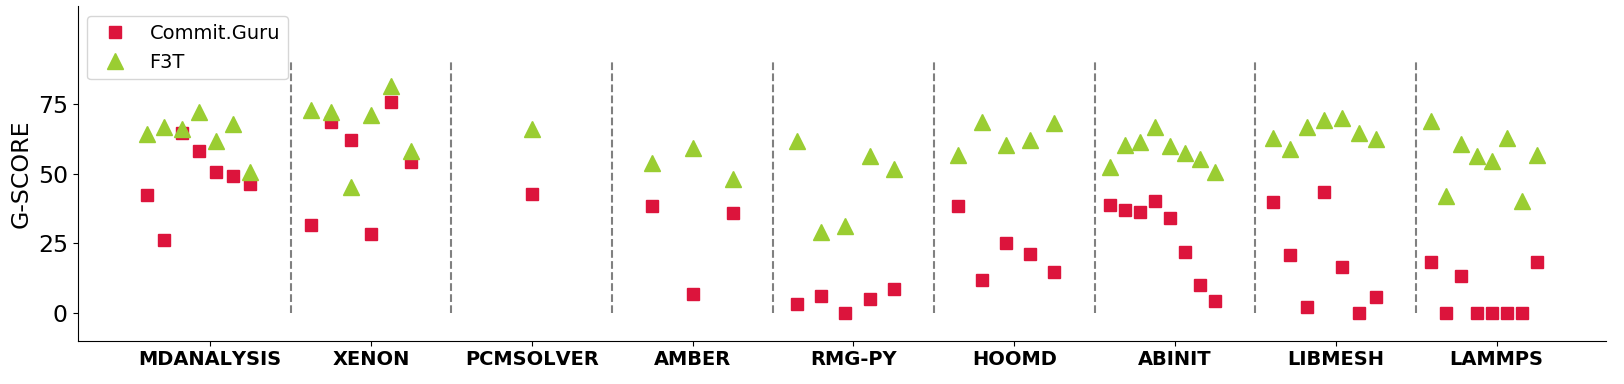
\includegraphics[width=.9\linewidth]{rq3_1.png}
\end{figure*}   


Nevertheless, if a widely used method only works well for certain software domains,
then it becomes an important  task to  
adapt those methods to other domains. 
Accordingly, this paper introduces  
$F^3T$
(short for ``FASTREAD and FAST FRUGAL TREES''),
a semi-automatic methods for labeling   Github issues (then using them to build 
 defect predictors). FASTREAD is an incremental 
{\em active learner} that  implement a human+AI partnership where humans read the {\em fewest} items in order to train a classifier that can detect the {\em most} number of interesting/worrying commits. Previously, FASTREAD has been used to help humans search $1,000$ papers in Google Scholar to find  the dozen or so that are most relevant to some   research query~\cite{Yu:2018}.
FAST FRUGAL TREES are a ensemble-based learner which has recently showed
much promise for software analytics ~\cite{di18_fft} (i.e. traditional defect prediction on release level).


%The central insight of this paper is that the commit labeling problem  is   analogous to reading research papers. Hence, an active learner like FASTREAD, which was designed for    reading research papers, could also be usefully deployed for handling commit messages. 
The central insight of this paper is that commit labeling  is  analogous to reading research papers and defect predicting of buggy commits is analogous to release-level defect predicting. Hence, an active learner like FASTREAD (designed for reading research papers) and FFTs (adapted from release-level defect prediction) would be useful for handling buggy commits identification and prediction.

 
To test the value of FASTREAD and FAST FRUGAL TREES
for  labeling Github commit messages,  we built software
defect predictors by labeling $45,000$ commits messages  ($36,000$ after pre-processing for analytics tasks) from nine computational software
projects  using (a)~the standard keyword method as implemented in the  Commit.Guru tool~\cite{commitguru} and (b)~active learning with $F^3T$.  
%To simulate real world constraints, we limit ourselves to what could be achieved with one week (40 hours) of work.

To structure this investigation, we ask four questions:
\newpage\noindent
{\bf RQ1: How close are FASTREAD and keyword labeling to human labels?}


This question compares  different labeling methods (keywords, FASTREAD)
against  ground truth labels (assigned by a team of humans).
 We will see that:

\begin{RQ}{Compared to keyword labeling...}
FASTREAD was best at reproducing the ground truth (i.e. the human labels).
\end{RQ}

% Manual labeling is a very labor intensive process. Hence, {\bf RQ1} was studied
% using   just a  subset of our data (four projects) while {\bf RQ2,RQ3}  used all our project data with
% the commit messages labelled
% by the best method found in {\bf RQ1}.   
%XXXX (Aside: For the new project data not studied by manual labeling,
% we applied the following sanity check. 5\% of the 
% commits, selected at random, from the new data was manually inspected. That sanity 
% showed that FASTREAD's labeling performed very well.)

\noindent
{\bf RQ2: Does keyword labeling lead to  better predictors for buggy commits? }

{\bf RQ1} only explored the labeling process.  
In {\bf RQ2}, we 
check how well those labels predict for defects.
For this research question, we kept the learner constant  (only FFTs) and varied
the labeling method (keywords or FASTREAD).
Project data
was divided into releases $r_1, r_2,... $ etc.
Classifiers were trained on release $r_i$ 
then tested on $r_{i+1}$. 
  We will see that:

\begin{RQ}{Compared to keyword labeling...} 
FASTREAD's   generated better   predictors for buggy commits.
\end{RQ}
  
  
\noindent
{\bf RQ3: What predicting method best predicts for buggy code?}

{\bf RQ2} built predictors using only one classifier (FFT). 
Now, for {\bf RQ3},  we used the labeling method endorsed
by {\bf RQ2} (FASTREAD) and varied
the data mining algorithm (FFTs versus the combination of the SMOTE preprocessor with logistic regression (LR), random forests (RF),
support vector machines (SVM)). 
 We will see that:

\begin{RQ}{Compared to other predicting methods...}
Of the predicting methods studies here, FFTs built the best classifiers for buggy commits.
\end{RQ}


{\bf RQ4: Which identification and prediction system perform best for buggy commits?}

This investigation is the comparison of our proposed  system or $F^3T$ versus the state-of-art system (i.e. Commit.Guru \cite{commitguru}) for identification and prediction system. Commit.Guru is tweaked at the last step to incorporate SMOTE while varying the choice of learners (LR, RF, and SVM) to cover top and bottom ranked categories recommended by Ghotra et al. \cite{ghotra15} building on top of the data generated by the keyword labeling method. 
We found that:

\begin{RQ}{Compared to the state-of-the-art system ...}

The proposed $F^3T$ outperformed the existing system buggy commits identification and prediction.

\end{RQ}
%(Note that \fig{rq3_1} shows   {\bf RQ3} results where FASTREAD+FFT
%labelled the commits in prior releases, then then classified other commits in subsequent releases.

In summary,
these results make us recommend $F^3T$ (FASTREAD + FAST FRUGAL TREES) for labeling Github
commit messages, then generating defect predictors. 
As shown \tion{iia},  this method can reduce the cost
of labeling Github commits by an order of magnitude.


\noindent
As to the novel contributions of this paper:
\be
\item This paper is the first to introduce $F^3T$ .
\item
To the best of our knowledge,
 this work  is the first to use active learners  to label  Github messages.
 As shown below, this combination of human+artificial intelligence is very useful since it
 quickly leads to better predictions.
\item
Much prior work in software defect prediction has used a small number of open source projects,
mostly written in JAVA~\cite{Fu2016TuningFS}.
This paper is the first report of applying a broad range of AI tools (active learners and classifiers)
to  empirical SE for an entirely different class of software (from computational science). 
\item 
To better support other researchers  
  our scripts and  data are  on-line
at github.com/sillywalk/defect-prediction/.
\ee
% \noindent
% In summary, the main contributions of this paper are:
% \bi
% % \\item 
% % \item Fastread labeling offer higher quality data for predicting risky software commit than state-of-the-art labeling method, Commit.Guru's automatic keyword labeling.  
% % \item FFTs as a recommended data mining model offer better improvement of performance scores than state-of-the-art methods, Commit.Guru's Logistic Regression. 
% \item A first novel inter-disciplinary contribution of human+AI partnership and psychological science in software quality assurance. 
% \item A demonstration of Human+AI partnership for software analytics outperforming approaches that are solely abusing AI. 
% \item An assessment of active learning for data ingestion quality problem by reproducing prior approach and comparing it with our recommended system.  
% \item A reproduction package containing all the data and algorithms of this paper, see \url{https://github.com/anonymous-for-review}.
% \ei
The rest of this paper is structured as follows. Background work is discussed  in the next section.
\S3 and \S4 describes our empirical methodology and experimental design.  This is followed by the details of the experiment used
to answer our research questions in \S5.
Further discussion, threats to validity, and  possible
future work from this research are explored in \S6, \S7, and \S8. Finally, conclusion of this work is given in \S9.
  
  Before beginning, we offer a comment about Commit.Guru~\cite{commitguru}. 
 Commit.Guru supports
  many  important features which we use extensively in this paper (e.g. the SZZ algorithm \cite{Kim08changes, Sliwerski05changes, costa17szz}, feature extraction from projects). 
  Hence, we strongly endorse the use of this tool (though its
   labeling and predicting methods should be improved).
  

 
  
  

  
%   regardless of studies showing low accuracy performance even with the help of topic modeling \cite{fu05committopic}. 
  
%  shows decisions of 15 commit messages and a lot of them can be incorrectly labeled by the traditional automatic
% keyword approach (i.e. looking for presence of the Table \ref{tab:words} terms in the commit message). 


%is a far more human-facing process which inherently

% \begin{figure}[!t]
% 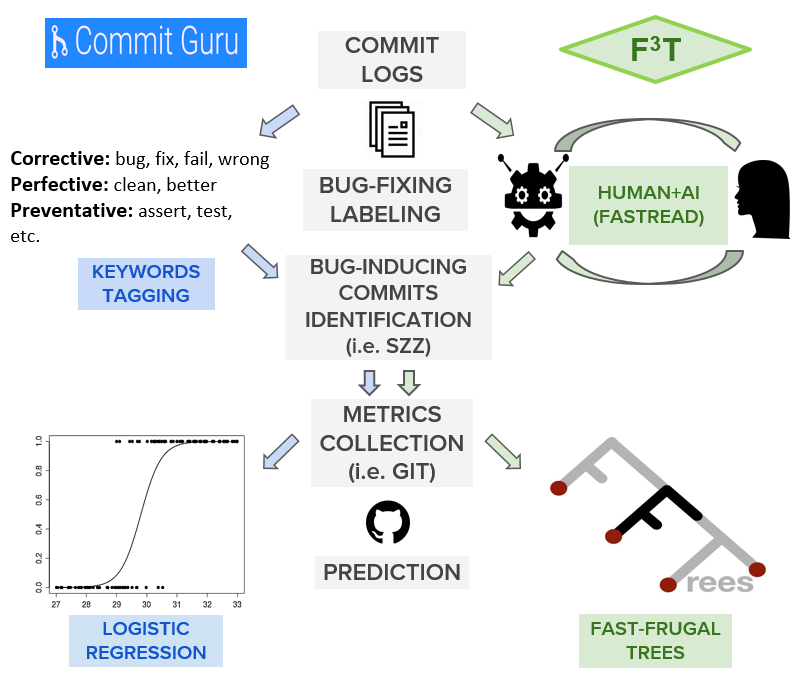
\includegraphics[width=\linewidth]{summary.PNG}
% \vspace{-14pt}
% \caption{Summarized data mining pipeline of $F^3T$ versus the state-of-the-art system (i.e. Commit.Guru \cite{commitguru}) for risky software commit prediction. Blue left flow represents Commit.Guru system while Green right flow represents our recommended system, $F^3T$.}\label{fig:system}
% \vspace{-6mm}
% \end{figure} 

%But how to capture human knowledge about what issues should be explored or ignored?
%Current practice it so use a



%These commit messages include specialized grammars and contents.
% Current practice of developers in software maintenance involved them describing these maintenance in commit messages.


% One important aspect of software maintenance is to find the defects within the software in order to allocate relevant resources to fix it and  approximate the trend how the defects occur for bettering future practices of software maintenance \cite{menzies10dp, menzies07dp, ambros10extensive, nagappan05codechurn,elbaum00codechurn, moser08changemetrics, hassan09codechanges}.  Due to the importance of defect prediction, numerous studies this past decade proposed methods to help identify defects. Researchers have analyzed source code (e.g., by code metrics or code smells) \cite{menzies07defect, menzies10dp, ambros10extensive}, or source code comments and commit messages introduced by a developer intentionally describing their work \cite{mockus00changeskeys, hindle08_largecommits, Kim08changes, kamei12_jit}. For e.g., one commit in the ABINIT project is ``        exttt{Fixed bug in DDB interpolation}'' indicates that the corresponding code was ``fixed'' just now to handle DDB interpolation. Therefore, before the patch of this issue got fixed, the previous code has bugs and researchers applied  (1) Sliwerski, Zimmermann, and Zeller algorithm (SZZ)  traced back the commit that introduced the bugs \cite{costa17szz, Kim08changes, Sliwerski05changes}, (2) collect the metrics associated with the bugs \cite{menzies07dp, commitguru, kamei12_jit}, (3) build defect predictors on them \cite{agrawal2018better, di18_fft, Tu18Tuning, ghotra15}. 
% Figure \ref{fig:system} shows this pipeline,
% bas instantiated by the Commit.Guru tool~\cite{commitguru} (illustrated as the blue flow). 

% %The premise of this paper is that, apart from the problem addressed by SZZ, there is {\em another} part of the Figure \ref{fig:system}  that deserves more attention.
% Most prior research in software analytics focuses on bug-inducing commits identification, metrics collection, and prediction (the later parts of the pipeline). The problem of automating labeling these commits in Table \ref{tab:words}  is rarely explored, even though this step is the primary task of Figure \ref{fig:system} to get the ``right'' data for consequent tasks. Current practice in software analytics is to categorize these commit messages via the set intersection of the text against a list of keywords (see Table \ref{tab:words}). Vasilescu et al. \cite{Vasilescu15github} remarked that this categorization process is central for researchers to generating defect prediction learning on changes level \cite{commitguru, Kim08changes, catolino17_jitmobile, nayrolles18_clever} regardless of studies showing low accuracy performance even with the help of topic modeling \cite{fu05committopic}. For instance, Table \ref{tbl:sample} shows decisions of 15 commit messages and a lot of them can be incorrectly labeled by the traditional automatic
% keyword approach (i.e. looking for presence of the Table \ref{tab:words} terms in the commit message).  It is timely to call for an empirical study for assessing and exploring the labeling process for software analytics, especially risky software commits prediction. Hence, this paper and our recommended system, $F^3T$ (illustrated as the green flow in Figure \ref{fig:system}).

 
 %``risky, not risky''\footnote{Which is Commit.Guru's way of denoting "buggy" or "not buggy".} 
 





%Deciding which commits are bug-fixing can be quite complex. 


 
 
%without exploring and assessing the labeling process which is the first and foremost step in the pipeline to collect the ``right'' data (i.e., bug-fixing commits as the first step in the pipeline). 


%They further remark that while the categorization process is central to tasks such as generating defect predictors, only few papers rigorously explore this categorization process. 
%The current trend of researching approaches include (1) tracing the right commit that introduces the bug (i.e. SZZ) \cite{costa17szz, Kim08changes, Sliwerski05changes} and (2) collecting bugs' metrics and building data miners \cite{yan18_tddetermination, kamei12_jit, nayrolles18_clever, catolino17_jitmobile, yan18_tddetermination, commitguru} 



%Moreover, , it is aligned with Agrawal et al. \cite{agrawal2018better} reported that fixing the weaker regions of the training data in SE defect prediction data can improve the performances on multiple criterias (e.g. AUC and recall drastically).

%This paper address the challenge raised by Vasilescu. We conducted a detailed examination of the process of categorizing comments to find that:

%\bi
%\item Purely automatic methods that just use keywords from Table \ref{tab:words} should be deprecated;
%\item Manual methods where humans reflect more on the commit messages and their categorization are recommended.
%\ei

% This work essentially addresses the challenges raised by Vasilescu et al. \cite{Vasilescu15github}. They recommended that the process is explored in an iterative manner where commit categories are studied manually as human engineers adjust the regular expressions containing these keywords.  We conducted a detailed examination of the process of categorizing comments to find that purely automatic method that merely uses syntactic criteria like  {\em words} from Table \ref{tab:words} can perform worse than the {\em combination} of Human+AI. At least in the particular case of studying textual artifacts from software projects, humans have more insight into those artifacts that AI.  More generally, we caution that humans should never be replaced by just AI algorithms. 





% That said,  adding humans into an analytic process is time-consuming. In the sample of commit messages explored by this study, commit messages are two to four lines long, and these can be read and critiques by humans at a rate of no more than ten per minute. This means that while automatic tools can read a billion commit messages in a minute, humans struggle to analyze ten. Hence, before we can advocate partnerships of human and artificial intelligence for software analytic, we must somehow manage and minimize the work required by the human partner.
 

\section{Motivation}

\subsection{Why Study Labeling?}\label{tion:iia}



For two reasons, we argue that it is important to study labeling. 
Firstly, there is the semantic issue.
As shown in \fig{rq3_1}, poor labeling leads to poor predictions. Other researchers also mention
that poor data quality (of both independent and dependent variables) can adversely effect prediction~\cite{herzig13_misclassifications,bird09_bias}.

Secondly,
% %the generation of correct labels is an essential 
% process for any analytics tasks that  needs
% a ground truth based on labelled issue commits
%   (such a ground truths are needed to train
%  and test a machine
% learning algorithm). 
% Much recent research~\cite{eirini15promise} builds this ground truth using data from
% Github
% (which is an on-line repository system holding  $10^7$ repositories of software projects and/or code).
% Neumann~\cite{neumann13} reports that in Github,
% the number of open issues can be twice the number of closed ones. In such projects, human maintainers are faced with more tasks than they can complete. Hence, their domain knowledge is required when deciding which issues are truly ``worrying''
% and which can be ignored. 
% One way to characterize this paper is a method for
% efficiently capturing that domain expertise.5555
labeling is a time consuming and expensive task. While most commit message are short\footnote{The sample  in \tbl{sample} reflects the median size of these messages.},   the  nine projects studied in this paper   have $45,000+$ (before  pre-processed) commits. Based on experience with running all-day data-labeling sessions (using  teams of graduate students), labeling these original $45,000+$ commit messages requires 225 person hours (or 25 hours on average for a project; median reading
times see in $5000+$ commits).  These nine projects are just a sample of the 59 computational science projects that
we have currently found on Github (and we suspect that an order of magnitude more such projects may exist).
Assuming these 59 projects have the same commit frequency as the nine, then labeling all 59 projects requires 37 weeks of work. Further,  if a second human is used to check the labels (which is standard practice
in manual SE research papers),  this estimate grows to 64 weeks (1.25 years).  And we are not finished yet. If any other research team wants to check our results (which is always good research practice) then yet another 1.25 years of may required (per secondary group), just to independently check those labeling.  


%While most commit message are short\footnote{The sample in \tbl{sample} reflects the median size of these messages.}, the nine projects studied in this paper \tbl{data} originally is $45000+$ commits. Based on experience with running all-day data-labeling sessions (using  teams of graduate students), we assert that labeling these  45,000 commit messages requires 40 to 80 person hours.  

% These nine projects are just a sample of the 55 computational science projects we can currently find on Github. We suspect that an order of magnitude such projects exist (and we have not found them yet). Assuming these 590 projects have  the same commit frequency as the nine, then labeling all requires  139 weeks of work. Further,  if a second human is used to check the labels,  this estimate grows to 260 weeks. 

What would it cost to complete all that labeling? The following estimates assumes
(a)~the   use of  crowdsourcing (via  Mechanical Turk);
(b)~our crowdworkers are being paid at least minimum age; and 
(c)~we assign two readers per issue report; 
(d)~a 50\% ``cull rate'' of crowd workers (where quality control questions are used to identify and prune  ineffective crowdworkers \footnote{Such a 50\% ``cull rate'' is common practice in crowdsourcincg~\cite{chen19}};
and (e)~and our university takes a 50\% overhead tax on grants. Under those assumptions,
 labeling 590 projects of Github issues would require  \$472K  of  grant money (with nothing left over for graduate student wages or other equipment).


But when using  $F^3T$, 
we would only need to read up to 16\% on median of the commits to find 95\% of the worrying commits.
That is, the same task would only consume  \$38K of grant money grant (which is an order of magnitude improvement). For details on how we make this calculation, see Table \ref{tbl:time1} and Table~\ref{tbl:time2}, later in this paper.

\subsection{Why Study Computational Software?}

The case studies of this paper come from computational science software. It is important to study such software since that code    has a widespread social impact.
For example, weather forecasts generated from computational science
software can   predict the path of hurricanes. This, in turn,
allows (e.g.) effected home owners to better protect themselves from
damaging winds. 
For another example, computational science explores the properties
of new materials. Synthesizing new materials is very expensive so standard practice is to use software to determine
those properties (e.g. via a finite element analysis). This, in turn, enables (e.g.) the faster transition of new materials to industry.
If better software engineering    improves computational
science software, then this would lead to better (e.g.) weather predictions and the faster creation of new industries based on new materials.

% Moreover, empirical SE has been mostly developed for tech giant (e.g. Facebook-, Google- and Microsoft-) style software. These three
% organizations
% are hardly representative of the vast
% ranges of  different software types in contemporary practice. The proposed system of this work could be used to better adapt empirical SE to Computational Science specifically but also to any other fields of endeavor. 


Another reason to study   computational science software  is that it can  be used to stress test
the generality of existing empirical SE methods.
Consider the results of \tbl{sample} and Figure \ref{fig:rq3_1} where a standard method  (keywords to identify worrying commit and traditional data miners derived from Ghotra et. al \cite{ghotra15}) failed very badly
when applied to computational science software.
This result is suggestive (but not conclusive) evidence that (a)~prior work on analytics has over-fitted
its methods (to systems like Apache);  and that (b)~it is 
now time to develop new case studies (like computational science).



\subsection{Why Study Defect Prediction?}

% The methods discussed in this paper would be useful for  
% any analytics
% task that studies commit message from software projects.
% Due to the space limitations of this paper, this paper focuses on just one of these tasks (defect prediction~\cite{menzies07precision})
% but other such tasks include  recognizing   software with security vulnerabilities~\cite{yu18v} or
% bad smells~\cite{KRISHNA201753}; 
% prioritizing  test cases~\cite{zhu2018test};
% or recognizing
% technical debt~\cite{huang2018identifying}.
  
%Software developers are smart, but sometimes make mistakes. Hence, it is essential to test software before the deployment ~\cite{orso2014software,barr2015oracle,yoo2012regression, myers2011art}. 
% From 1972 responses survey of Hannay et al. \cite{hannay09_secs}, 30-40\% of computational scientists time are devoted to develop and use scientific softwares. Yet, few of these scientists are trained in software engineering \cite{johan18_secs}. By default, scientists spent more than half of their programming time on finding and fixing errors of the software and only employing primitive debugging and testing methods (``if the output matches what I expected'') according to Prabhu et al. \cite{Prabhu11_cssurvey}. Software testing and software verification skills are judged important but scientists’ skills for these are lacking which leads to poor execution of both skills according to the survey studies done by Prabhu et al. and Carver et al. \cite{Prabhu11_cssurvey, heaton15_lit}. Hence, it is essential to test software before the deployment ~\cite{orso2014software,barr2015oracle,yoo2012regression, myers2011art}. 

 Software quality assurance budgets are finite while assessment effectiveness increases exponentially with assessment effort~\cite{Fu2016TuningFS}. Therefore,  standard practice is to apply  slower  methods on code sections that seem most critical or bug-prone.
Software bugs are not evenly distributed across the project~\cite{hamill2009common,koru2009investigation, ostrand2004bugs,misirli2011ai}.  Hence, 
a useful way to perform software testing is to allocate most assessment budgets to
the more defect-prone parts in software projects.    Data mining algorithms can input
features extracted from source code and output predictors for where defects are likely to occur.
Which such  predictors are never 100\% correct,
they can  suggest where to focus more expensive methods. 



There is  much  commercial interest  in  defect prediction.  In a survey of  395 practitioners from 33 countries and five continents,
 Wan et al.~\cite{wan18} found that over 90\% of
 the respondents were willing to adopt defect prediction
 techniques. 
 
  Results from commercial projects show the benefits of defect prediction.
 Misirli et al.~\cite{misirli2011ai} built a  defect prediction model  for a telecommunications company. Their  models
  predicted 87\% of code defects and   decreased inspection efforts by 72\% (while  reducing post-release defects by 44\%).  Kim et al.~\cite{kim2015remi} applied defect prediction model, REMI, to API
development process at Samsung Electronics.
They models  could
predict the bug-prone APIs with reasonable accuracy~(0.68 F1 score) and reduce the resources required for executing test cases.



Software defect predictors not only save labor compared with traditional manual methods, but they are also competitive with certain automatic methods.  
 Rahman et al. ~\cite{rahman2014comparing} compared (a) static code analysis tools FindBugs, Jlint, and PMD with (b) defect predictors (which they called ``statistical defect prediction'') built using logistic  regression.
No significant differences in   cost-effectiveness were observed.

Given this equivalence, it is significant to
note that  defect prediction can be quickly adapted to new languages by building lightweight parses to extract  code metrics. The same is not true for static code analyzers - these need extensive modification before they can be used in new languages.
Because of this ease of use,  and its applicability to many programming languages, defect prediction has been   extended  many ways including:
\be
\item Application of defect prediction methods to locating code with security vulnerabilities~\cite{Shin2013}.
    \item Predict the location of defects so that appropriate resources may be allocated (e.g.~\cite{bird09reliabity})
    \item Understand the factors that lead to greater likelihood of defects such as defect prone software components using code metrics (e.g., ratio comment to code, cyclomatic complexity) \cite{menzies10dp, menzies07dp, ambros10extensive} or process metrics (e.g., number of changes, recent activity) \cite{nagappan05codechurn,elbaum00codechurn, moser08changemetrics, hassan09codechanges}. 
    \item Use   predictors to proactively fix  defects~\cite{kamei16_lit, legoues12_aprlit, arcuri2011practical}
    \item Study defect prediction not only just release-level \cite{di18_fft, agrawal2018better} but also change-level or just-in-time \cite{yan18_tddetermination, kamei12_jit, nayrolles18_clever, commitguru} both for research and also industry.  
    \item Explore ``transfer learning'' where predictors from one project are applied to another~\cite{krishnaTSE18,nam18tse}.
    \item Explore the  trade-offs between 
    explanation and performance of defect prediction models~\cite{di18_fft}.
    \item Assess   different learning methods for building models that predict software defects~\cite{ghotra15}. This has led to the development of hyperparameter optimization and better data harvesting tools \cite{agrawal2018wrong, agrawal2018better, Fu17easy, Fu16Grid, Fu2016TuningFS,tantithamthavorn2016automated}. 
\ee
 The important thing to note about all these eight research areas is that  all their conclusions are wrong if commit
 message are labelled incorrectly.
 This is a concern since,  as  \tbl{sample} and \fig{rq3_1}
 showed, commit labeling
 can go very wrong if the wrong labeling methods is applied.
 

% \subsection{Defect Prediction: Details}

% For defect prediction to work on Github data, the following four step pipeline has to be created. 

% \subsubsection{Step1 = feature extraction}: extract features from numerous number of projects. 
% One challenge with handling code from multiple projects is
% that they may use different programming languages. For
% that reason, one modeling heuristic is to use language agnostic measures.
% Another heuristic, endorsed by
% Herslab~\cite{Tsay:2014} and Devanbu~\cite{Rahman:2013}, is to
% include as much information about (a)~the humans changing
% the code as (b)~the code itself. Both these
% heuristics are used by the  Commit.Guru tool~\cite{commitguru}. \tbl{metrics}
% shows the information that this tool can automatically extract from Github repositories.  Note that  the features in \tbl{metrics} divide almost equally into information about the code and information about how
% humans are changing that code.

% \subsubsection{Step2 = commit labeling}: Machine learners learn
% models that report what combination of {\em independent 
% features} predict for the {\em dependent features}.  In this paper, when we label a commit, we are defining the dependent variables.
% As seen  in Table~\ref{sample} and \fig{rq3_1}, 
% identifying which commit messages refer to bugs can  be an error-prone process (and the goal of this paper is to reduce such errors).


% \subsubsection{Step3 = blaming}:
% Once the above two steps are completed, then 
% a mapping must be built between the dependent labels as ``buggy'' (from Step1) and
% their associated independent features (from Step2).
% This is called    ``blaming''. 

% For that purpose, we use        
% Sliwerski, Zimmermann, and Zeller's SZZ's
%  algorithm~\cite{costa17szz, Kim08changes, Sliwerski05changes}.
%  to work back in time to  identify what code changes lead to the bug report.
%   Rodríguez-Perez et al.~\cite{RODRIGUEZPEREZ2018164}
%  report that at least 187 papers have also used SZZ
%  for that purpose. Due to the foundational role of SZZ,  recently  research has explored  ways
%  to better evalaute and better improve that algorithm (for more details on that, see~\cite{7588121}).

% \subsubsection{Step4 = induction}: Once Step3 completes, there is now a table of data with many
% independent columns and on depednet 

  
    

% Following the advice of~\cite{fu2018building,di18_fft,phillips2017fftrees}, for all the experiments of this paper, we use a depth    $d=4$. 
% For trees of depth $d=4$, there are $2^4=16$ possible trees which can be denoted as 00001, 00010, 00101, ... , 11110. During FFTs training, all $2^d$ trees are generated, then we select the best one (using the training data).
%  This single best tree is then applied to the test data.
%  Note that FFTs of such small
% depths are very succinct
% (e.g. Figures~\ref{fig:fft1}). Such FFTs generate rules which leads to decision of finding a report as risky or not risky (defective and non-defective) for the datasets under this study. Chen et al. reported that in comparisons to other standard models in software analytics (SVM, RF, LR, and NB), FFTs performed better in term of $P_{\mathit{opt}}$ and distance to the ``heaven'' point of 100\% recall and no false alarms in at least defect prediction and issue close time prediction  \cite{di18_fft}. Therefore, it is adopted and validated in our study in RQ2 for risky software commit prediction. 

% \begin{table}
% \small
% \begin{center}
% \caption{Dataset statistics. Data was mined and curated from each own open project's github repository.}
% \vspace{-10pt}

% \label{tbl:dataset}
% \begin{tabular}{c@{~}|r@{~}|r@{~}|r@{~}|r@{~}}
% \begin{tabular}[c]{@{}c@{}} \end{tabular} & \begin{tabular}[c]{@{}c@{}}         extbf{No. of}\end{tabular} &         extbf{No. of} &         extbf{Defective}  \\
%          extbf{Dataset} &         extbf{Commits} &         extbf{Releases} &          extbf{Commit \%} &         extbf{Source}\\ \hline
% HOOMD & 3904 & 6  & 16 & \cite{hoomd} \\ 
% LIBMESH & 7801 & 8 & 16 & \cite{libMesh} \\
% ABINIT & 3911 & 9 & 18 & \cite{Abinit} \\  
% LAMMPS & 5587 & 7 & 18 & \cite{lammps-sandia} \\ 
% PCMSOLVER & 1655 & 2  & 23 & \cite{pcmsolver}  \\ 
% AMBER & 4243 & 4  & 23 & \cite{Amber-MD} \\ 
% RMG-PY & 4472 & 7 & 27 & \cite{ReactionMechanismGenerator}  \\ 
% MDANALYSIS & 2733 & 8  & 37 & \cite{mdanalysis}  \\  
% XENON & 1804 & 7  & 46 & \cite{xenon} \\ 


% \end{tabular}
% \end{center}
% \vspace{-10pt}
% \end{table}


  

\section{ Incremental Active Learning}

  The case was made above that (a)~labeling commit messages is a vital task at the core of much current research; and (b)~manually labeling those commits is a very slow process. This
section describes the FASTREAD  active learning method
that incrementally labeling a small subset of the commits. Using those labels, a machine learner can then find nearly all the  remaining interesting/worrying commits. Using these methods, humans have to read in details only a small percentage of the commits (under 16\%, median value).  
 
% In this 
% Through software development and maintenance, developers are supported to describe their work that were pushed through commit messages. One popular practice of identifying or reasoning the rate of bugs is searching for defect-related keywords through these messages \cite{mockus00changeskeys, hindle08_largecommits}. It has been adopted in empirical SE research extensively without rigorous critique (e.g., \cite{nayrolles18_clever, catolino17_jitmobile, kamei12_jit, Kim08changes}). Does this set of keywords can be generalized to the diverse community of SE research? 

% According to Fu et al., even with the full automation through topic modeling, the accuracy performance was low \cite{fu05committopic}. For instance, this study specifically focuses on softwares from computational science (which is elaborated more in section 3.1) and Keyword automatic labeling method that have performed well in SE researches \cite{commitguru, nayrolles18_clever, Kim08changes, kamei12_jit} made fatal mistakes as recorded in Table \ref{tbl:sample}. There are indeed agreements between state-of-the-art keywords labeling and human+AI (i.e. FASTREAD column) that can be observed in the first 5 entries of Table \ref{tbl:sample}. However, for ``        exttt{Make error message clearer in tests for TPR parser}'' would be marked as bug-fixing commit and the commit introduces the code that being changed will be marked as buggy and the data miner will learn not relevant metrics to identify risky commit, which is a false-positive example. Moreover, such commits as ``        exttt{NetCDFWriter working (closes Issue 109)}'' was not marked as bug-fixing commit by the state-of-the-art keywords but it was indeed a bug-fixing one so the data associated with risky commit was not collected and learned for the data miner, which is a false-negative example. These mistakes conjectured that the standard Keyword automatic labeling in SE failed to fully capture the semantics of these commits. 
% Instead of going for full-automation for too low of relevancy or full-human for too expensive of labor work, the data ingestion and other studies \cite{costa17szz, Kim08changes, nayrolles18_clever, catolino17_jitmobile, kamei12_jit, kamei12_jit} that utilize it can improve by combining both manual and automating approaches for identifying bug-fixing commits, human-in-the-loop AI or human+AI partnership.
%  In the  nomenclature of \tbl{formal}, FASTREAD
%  starts with $L = \emptyset$ commits (i.e. nothing labelled, no commits read). Next, it
% prioritizes which commits to be reviewed in order to   maximize $|L_{R}|$ (the number of relevant or bug-fixing commits discovered)
% while minimizing $|L|$ (number of commits reviewed).

%ctive learners like FASTREAD are AI  tools that
% explore a large code base to find commits that seem most likely to be
% interesting or
% worrisome~\cite{Cormack2017Navigating, Cormack2016Engineering, cormack2016scalability, Cormack2015Autonomy, Cormack2014Evaluation, Wallace2010Semi, wallace2010active, wallace2011should, wallace2012class, nguyen2015combining}.  Next, humans apply their  expertise  to review that guess by either
% agreeing or disagreeing that it is worrisome (and, if the latter, then
% the  active
%  learner  the support vectors of  a SVM learner).
%   The experience outside of SE is that  machine learning algorithms can train faster (i.e. using less data) if it is allowed to choose the data from which it learns~\cite{settles2012active} (but to avoid over-fitting, 
%  we ensure in         \tion{eval} that the results
%  of that training  process is  tested on data {\em not} seen during  training). Active learning has not been extensively explored
%  within SE and, to the best of our knowledge, it has not been 
%  previously applied
%  to the commit labeling problem.
% In order to achieve the combination, {\em active learning} is adapted. It can train faster (i.e. using less  data) if it is allowed to choose the data from which it learns~\cite{settles2012active}. The experience in other domains in literature reviewing task (e.g. legal reasoning, evidence-based medicine, and software engineering) is that such active learners can significantly reduce the amount of effort required to achieve high recall~\cite{Cormack2017Navigating, Cormack2016Engineering, cormack2016scalability, Cormack2015Autonomy, Cormack2014Evaluation, Wallace2010Semi, wallace2010active, wallace2011should, wallace2012class, nguyen2015combining, Yu2018Recall}. Systematic literature review specifically in SE is a manual process till recent development of automatic tool support FASTREAD that utilize active learning. 


 \begin{wrapfigure}{r}{1.4in} 
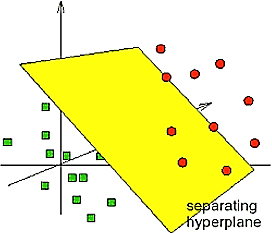
\includegraphics[width=1.4in]{svm.png}
 \caption{ Separating worrying (red) from  non-worrying (green) files.}\label{fig:svm}
 \end{wrapfigure}To understand   active learning,  consider the decision boundary between the worrying commits and 
 other commits shown in \fig{svm}. 
 One tactic for quickly
 finding those worrying commits would be to ask humans to review and assess a few dozens of commits that fall into the red region of this figure, as far as possible from the green ones (i.e. {\em certainty sampling}). Another tactic would be to review items that are closest to the boundary (i.e. {\em uncertainty sampling}). 
 
\begin{table}[!b]
\footnotesize
\caption{Problem description for FASTREAD.}\label{tbl:formal} 
\label{tab: problem}
\begin{tabular}{ll}
\rowcolor{gray!10} 
$E$: & the set of all candidate commits (in the project).\\\rowcolor{gray!10} 
$R\subset E$: & the set of ground truth worrying commits. \\\rowcolor{gray!10} 
$I=E\setminus R$: & the set of ground truth not worrying commits.\\\rowcolor{gray!10} 
$L\subset E$: & the set of labeled/reviewed commits, \\\rowcolor{gray!10}  & each review reveals whether a commit $x\in R$.\\\rowcolor{gray!10} 
$\neg L=E\setminus L$: & the set of unlabeled/unreviewed commits.\\\rowcolor{gray!10} 
$L_R=L\cap R$: & the identified worrying (included) commits.\\\rowcolor{gray!10} 
$L_I=L\cap I$: & the identified not worrying (excluded) commits.
\end{tabular} 
\end{table}
 



  All these tactics are built into FASTREAD~\cite{yu18v},
 the active learner used for this work.
 When reading   commits, FASTREAD
 initially uses uncertainty sampling to fast build a classification model (for ``worrying''
 or ``non-worrying'' commit message), then switches to certainty sampling to greedily find worrying commits. The machine learner (i.e. SVM) use this feedback from human to learn their models incrementally. These models are then used to sort the stream of commit messages such that humans read the most informative ones first
 (and the commits are resorted each time a human offers a new label for a commit). More specifically, 
 FASTREAD executes as follows (and this description uses the  nomenclature of \tbl{formal}):
 \bi
 \item
 FASTREAD executes by presenting to a human,  one example at a time. Whenever a human
offers a label to an example, FASTREAD updates an SVM model.
\item
More specifically, FASTREAD starts by
randomly sampling unlabeled candidate studies until humans declare that they see $N_1=1$ relevant examples. In 
the context of this paper,  ``relevant'' will
mean ``worrying commit''.
\item
Then, FASTREAD
start training with weighting to control query with uncertainty sampling, until $N_2=30$ relevant examples are found.
Here, different weights are assigned to each class
($W_R= 1/|L_R|$, $W_I= 1/|L_I|$).
\item
Next, FASTREAD trains  further  using
certainty sampling and 
Wallace's ``aggressive undersampling'' ~\cite{Wallace2010Semi}
that culls   majority class examples closest to the  decision boundary.
\item 
FASTREAD
stops training when it is estimated that \mbox{$N_3=95\%$} of the relevant have
been found.
\ei


\begin{table*}[!t]
\caption{Data used in this study.}\label{tbl:data}
\vspace{-5pt}
~\hrule~
\vspace{1.5mm}

\begin{minipage}{.45\linewidth}
{\bf         \tbl{data}a: Data selection and pruning.}
 
%{\normalsize 
 
678 computational science projects were identified.
Many of these are purely personnel projects (or just used for web storage)
so following the advice of Kalliamvakou et al.~\cite{Kalliamvakou:2014}, we used the sanity
checks of         \tbl{data}b to prune these  to 59 projects.
On these, we  use nine  (selected to cover a range of languages):
\bi
\item PCMSOLVER:   API to the Polarizable Continuum Model \cite{pcmsolver}.
\item XENON: middleware      interface to  compute \& storage resources \cite{xenon}.

\item MDANALYSIS: Python code to analyze molecular dynamics trajectories generated  from other simulation packages \cite{mdanalysis}.
\item  HOOMD:  particle simulation  for  hard particle Monte Carlo simulations of a many shape classes  \cite{hoomd}.  
\item ABINIT  : an atomic-scale simulation software suite \cite{Abinit}.
\item  AMBER: Fast, parallelized molecular dynamics   analysis \cite{Amber-MD}.

\item  RMG-PY: the Python Reaction Mechanism Generator.  Generates chemical reaction mechanisms for modeling reaction systems \cite{ReactionMechanismGenerator}.
\item LAMMPS: Large-scale Atomic/Molecular Massively Parallel Simulator, a classical molecular dynamics simulation code \cite{lammps-sandia}.
\item LIBMESH:   numerical simulation of partial differential equations   on serial and parallel platforms.  \cite{libMesh}.
\ei
For statistics on these systems, see         \tbl{data}c.

\end{minipage}~~~~\begin{minipage}{.55\linewidth}
 \begin{center}
{\bf    \tbl{data}b: Sanity checks (designed using~\cite{Kalliamvakou:2014}).}


{\scriptsize
 \begin{tabular}{r|l}
\rowcolor{gray!30}Check   & Condition    \\\hline
Personal purpose (\# Developers) & $>$ 7 \\
Collaboration (Pull requests)  & $>$ 0 \\
Issues & $>$ 10 \\
Releases &  $>$ 1 \\
Commits & $>$ 20 \\
Duration  & $>$ 1 year 
\end{tabular}}


 \vspace{10mm} 

{\bf        \tbl{data}c: Statistics on selected systems.}

 

\resizebox{.95\linewidth}{!}{
\begin{tabular}{r@{~}|r@{~}|r@{~}|r@{~}|r@{~}|r@{~}|r@{~}}
% \begin{tabular}[r]{@{}c@{}}   \end{tabular} & \begin{tabular}[c]{@{}c@{}}  \end{tabular} & \begin{tabular}[c]{@{}c@{}}\rowcolor{gray!30}         extbf{Duration} \end{tabular} & \begin{tabular}[c]{@{}c@{}}         extbf{No. of} \end{tabular} & 
% \begin{tabular}[c]{@{}c@{}}         extbf{No. of}\end{tabular} &         extbf{No. of} &         extbf{Buggy}  \\
%         extbf{DATASET}&        extbf{Language} &         extbf{(years)} &         extbf{Developers} &         extbf{Commits} &         extbf{Releases} &          extbf{Commit \%} \\ \hline
\rowcolor{gray!30}        & & Duration & No. of & No. of     & No of.    & Buggy\\
\rowcolor{gray!30} Dataset & Language & (years) & Developers & Commits & Releases & Commit\%\\\hline
HOOMD & C++ & 3 & 41 & 3904 & 6  & 16 \\ 
LIBMESH & C & 6.5 & 56 & 7801 & 8 & 16 \\
ABINIT & Fortran & 2.5 & 23 & 3911 & 9 & 18  \\  
LAMMPS & C++ & 5.5 & 84 & 5587 & 7 & 18 \\ 
PCMSOLVER & C++ & 4.5 & 8 & 1655 & 2  & 23  \\ 
AMBER & C++ & 4.5 & 11 & 4243 & 4  & 23 \\ 
RMG-PY & Python & 9.5 & 47 & 4472 & 7 & 27   \\ 
MDANALYSIS & Python & 4 & 80 & 2733 & 8  & 37  \\  
XENON & Java & 6 & 11 & 1804 & 7  & 46  \\ 
\end{tabular}
}

\end{center}
\end{minipage} 
\vspace{1.5mm}
~\hrule~
\end{table*}

% \begin{table*}[!t]

% ~\hrule~ 

% \begin{center}
% {\bf         \tbl{data}a: Data selection and pruning.}
 
% %{\normalsize 
%  \begin{tabular}{p{5in}}
% 678 computational science projects were identified.
% Many of these are purely personnel projects (or just used for web storage)
% so following the advice of Kalliamvakou et al.~\cite{Kalliamvakou:2014}, we used the sanity
% checks of         \tbl{data}b to prune these  to 55 projects.
% On these, we  use nine  (selected to cover a  range of languages):
% \bi
% \item PCMSOLVER:   API to the Polarizable Continuum Model \cite{pcmsolver}.
% \item XENON: middleware      interface to  compute \& storage resources \cite{xenon}.

% \item MDANALYSIS: Python code to analyze molecular dynamics trajectories generated  from other simulation packages \cite{mdanalysis}.
% \item  HOOMD:  particle simulation  for  hard particle Monte Carlo simulations of a many shape classes  \cite{hoomd}.  
% \item ABINIT  : an atomic-scale simulation software suite \cite{Abinit}.
% \item  AMBER: Fast, parallelized molecular dynamics   analysis \cite{Amber-MD}.

% \item  RMG-PY: the Python Reaction Mechanism Generator.  Generates chemical reaction mechanisms for modeling reaction systems \cite{ReactionMechanismGenerator}.
% \item LAMMPS: Large-scale Atomic/Molecular Massively Parallel Simulator, a classical molecular dynamics simulation code \cite{lammps-sandia}.
% \item LIBMESH:   numerical simulation of partial differential equations   on serial and parallel platforms.  \cite{libMesh}.
% \ei
% For statistics on these systems, see         \tbl{data}c.
% \end{tabular}

%  \vspace{10mm} 

% {\bf    \tbl{data}b: Sanity checks (designed using~\cite{Kalliamvakou:2014}).}


% {
%  \begin{tabular}{r|l}
% \rowcolor{gray!30}Check   & Condition    \\\hline
% Personal purpose (\# Developers) & $>$ 7 \\
% Collaboration (Pull requests)  & $>$ 0 \\
% Issues & $>$ 10 \\
% Releases &  $>$ 1 \\
% Commits & $>$ 20 \\
% Duration  & $>$ 1 year 
% \end{tabular}}


%  \vspace{10mm} 

% {\bf        \tbl{data}c: Statistics on selected systems.}

 
% \begin{tabular}{r@{~}|r@{~}|r@{~}|r@{~}|r@{~}|r@{~}|r@{~}}
% % \begin{tabular}[r]{@{}c@{}}   \end{tabular} & \begin{tabular}[c]{@{}c@{}}  \end{tabular} & \begin{tabular}[c]{@{}c@{}}\rowcolor{gray!30}         extbf{Duration} \end{tabular} & \begin{tabular}[c]{@{}c@{}}         extbf{No. of} \end{tabular} & 
% % \begin{tabular}[c]{@{}c@{}}         extbf{No. of}\end{tabular} &         extbf{No. of} &         extbf{Buggy}  \\
% %         extbf{DATASET}&        extbf{Language} &         extbf{(years)} &         extbf{Developers} &         extbf{Commits} &         extbf{Releases} &          extbf{Commit \%} \\ \hline
% \rowcolor{gray!30}        & & Duration & No. of & No. of     & No of.    & Buggy\\
% \rowcolor{gray!30} Dataset & Language & (years) & Developers & Commits & Releases & Commit\%\\\hline
% HOOMD & C++ & 3 & 41 & 3904 & 6  & 16 \\ 
% LIBMESH & C & 6.5 & 56 & 7801 & 8 & 16 \\
% ABINIT & Fortran & 2.5 & 23 & 3911 & 9 & 18  \\  
% LAMMPS & C++ & 5.5 & 84 & 5587 & 7 & 18 \\ 
% PCMSOLVER & C++ & 4.5 & 8 & 1655 & 2  & 23  \\ 
% AMBER & C++ & 4.5 & 11 & 4243 & 4  & 23 \\ 
% RMG-PY & Python & 9.5 & 47 & 4472 & 7 & 27   \\ 
% MDANALYSIS & Python & 4 & 80 & 2733 & 8  & 37  \\  
% XENON & Java & 6 & 11 & 1804 & 7  & 46  \\ 
% \end{tabular}


% \end{center} 
% ~\hrule~
% \caption{Data used in this study.}\label{tbl:data}
% \end{table*}


 
To generate the $N_3$ estimate,
whenever the SVM  model  is retrained, FASTREAD makes temporary ``guesses''  about 
 the unlabeled examples (by running those examples through the classifier).
 To turn these guesses into an estimate of the remaining worying commits, FASTREAD:
 \be
 \item 
 Builds  a  logistic  regression  model, using the guesses.
 \item
 Using  that regression model, FASTREAD makes new guesses on the remaining unlabelled examples.
 \item
 Loops back to step1 until the new guesses are the same as the guesses
 in the previous loop.
 \item
 Uses this logistic regression model to estimate
 the remaining number of positive examples in the data. 
 \ee
The reader will note that there are many specific  requirements built into the above
decisions (e.g. the values   $\{N_1=1, N_2=30, N_3=95\%\}$). Those requirements where made by 
 Yu et al.~\cite{yu18v} after exploring 32 different kinds of  active learners.
 They report that, using the above requirements,
 FASTREAD
 found  more relevant items faster than the
previously reported state-of-the-art in incremental text mining
retrieval~\cite{wallace2010active, Cormack2015Autonomy}. Further,
the $N_3$ estimator converged much faster and obtained better estimates
that  other prominent  estimators from the text mining literature~\cite{ros2017machine,Cormack2016Engineering,wallace2013active}.


 
 Yu et al.~\cite{yu18v} designed FASTREAD to help filter research papers from Google Scholar.
The central insight of this paper is that the commit labeling problem  is  analogous  to  reading  research  papers.  Hence, an  active  learner  like  FASTREAD
(which  was  designed  for reading research papers) could also be usefully deployed for handling commit messages. 

Our pre-experimental belief was that FASTREAD
would require extensive tuning before it could be  used for labeling
    Github commits. This was not true.  The following results were obtained
using Yu et al.'s original decision decisions \cite{yu18v}. 


% \subsection{Defect Prediction Past and Now}

% In 2007, the market for software tools and services has been growing to \$300 million, with 50 to 83 percent increases in static analysis and black-box testing sectors. More robust and secure software is necessary as this trend continues. Software faults and
% failures were estimated by the US National Institute of
% Standards and Technology (NIST) that  \$60 billion a year in the US \cite{softwareecon}. 

% Therefore, significant SE research has focused on software analytics and the prediction of software quality. Data about the development process (e.g., code and/or repository data) is trained to provide software analytics. In fact, in the past decade more than a hundred paper were published on software defect prediction alone \cite{sedp100}. Consequently, detecting the existence of defects in software projects an evergreen research field with 5 popular research paths:


% \subsection{Risky Software Commit Prediction}

% Previous studies have focused on the prediction of risky software changes for short-term quality assurance. Mockus and Weiss predicted the risk of a software change at coarse-grained granularity in an industrial project with features such as \# of subsystems touched,\# of files modified, \# of modification requests. Through studying defect-introducing changes in the Mozilla and Eclipse, Sliwerski \cite{Sliwerski05changes} found that large transaction of code would include defect and changes done on specific time have a higher change of introducing defects, especially Friday. Eyolfson et al. \cite{Eyolfson11bugginess} noted that software changes performed late night (between midnight and 4 AM) are more buggy than changes committed morning (7 AM and noon) and that developers who commit regularly produce less buggy changes.  A study
% that characterizing incorrect defect fixes in Linux, OpenSolaris, FreeBSD, and a commercial operating system by Yin et al. \cite{Yin11fixes} found that 14.8\%-24.2\%  of fixes are incorrect and affect end users, that concurrency defects are the most difficult to fix, and that developers responsible for incorrect fixes usually do not have enough knowledge about the code being changed.

% Inspired by their work, Kamei et al. \cite{kamei12_jit} completed a large scale study of the Just-in-time (JIT) software change on a set of 6 open source projects and 5 commercial projects through the 14 metrics categorized into 5 dimensions of diffusion, size, purpose, history, and experience. To the most recent work, Kim et al. \cite{Kim08changes} sampled a balanced subset of changes and use source code change logs in several open source projects and obtained 78 percent
% accuracy and a 60 percent recall. However, Kamei's work use the combination of change logs and the change metrics, reported in Table \ref{tbl:metrics}, predicting defect-inducing chnages with 68\% accuracy and 64\% recall with lower fraction bug inducing changes. 
% Barnett et al. extended Commit.Guru to include commit volume and Naive-Bayes (NB) score on how risky a commit content is on 342 MSR coding data challenge repositories to incorporate the relationship between commit message detail and defect pronerective, adaptive, or perfective issues \cite{barnett13_mcontent}.  

% Rosen et al. developed by a tool called Commit.Guru ~\cite{commitguru} to identify ``risky'' commits have made change-level defect prediction research path more accessible (the system is described in the blue flow of Figure \ref{fig:system}). They categorized actions undertaken by commits based on a list of verbs present in the messages into five categories (a) corrective action, (b) feature addition, (c) merge, (d) documentation, and (e) perfective and preventative measures. The LR model is used for classification task by building it on top of  stemmed from prior work  that are shown in Figure \ref{tbl:metrics}. 
 
% Previous work have sparked change-level bug level in different domains in software analytics. In 2017, Catolino \cite{catolino17_jitmobile} evaluated metrics proposed by Kamei et al. \cite{kamei12_jit} for JIT bug level for mobile applications domain with 5 open-source mobile applications where they found only a subset of 5 metrics were considered meaningful including: \# modified subsystems, \# added LOC, \# LOC before the commit, \# developers working on the committed files, experience of the developer. Through LR for modeling, they achieved 70\% accuracy but 17\%-38\% for recall. In 2018, Nayrolles et al. \cite{nayrolles18_clever} extends Commit.Guru to build the CLEVER (Combining Levels of Bug Prevention and Resolution techniques) tool experimenting on 12 Ubisoft software projects to help repair the program more proactively. Instead of LR, they classify the commit risky or no-risky based on Random Forest algorithm. If the commit is risky, they then comparing commit code blocks with NICAD code clone detector \cite{cordy11_NiCad} of software clones with similar defect-introducing commit and proposed the associated bug-fixing commit as the potential fix to the developer. Yan et al. \cite{yan18_tddetermination} studied 7 projects at change-level for technical-debt (TD) introducing changes of Hadoop, Ant, Camel, Jmeter, Log4j, Tomcat, and Gerrit from 0.75\% to 4.22\% targeted TD-introducing changes. They extended 13 features studied by Kamei et. al \cite{kamei12_jit} to 25 changes features categorized into Diffusion, History, and Message with $FA, FM, FD, FR, FC$, $LCC, MCC, HCC,$ and $CCC$ calculated by ChangeDistiller \cite{fluri07_changedistiller}. They applied NB and RF model to train and determine TD-introducing changes. Diffusion is the most discriminating features set to learn TD-introducing changes with AUC score of 82\% and cost-effectiveness of 80\%.


% From all of the above work, we noticed: 
% \begin{enumerate}
%     \item None questioning the full automation nature of dependent feature acquisition (bug-fixing commits identification through keyword tagging), i.e. buggy or non-buggy software changes for risky commit prediction model. Barnett et al. found that 43\% and 80\% of the JIT models of the studied systems are significantly improved by incorporating the relationship between commit message detail and defect proneness \cite{barnett13_mcontent}. Yet, independent metric FIX and bug-fixing status of a commit (for future tracing the risky software commits as the targets) are done by automatically searching for the existence of the defect-related keywords in the commit messages even when discouraged by low performance with support of topic modeling. Our work shall augment the bug-fixing status of the commits by FASTREAD method to improve the quality of dependent features of the risky software change prediction data. 
%     \item Only the large scale study done by Kamei et al. \cite{kamei12_jit} mentioned how to deal with imbalance class problem nature of defective change-level prediction by resampling approach to randomly delete instances from the majority category. Our experiment will incorporate state-of-the-art imbalance class handling technique, Synthetic Minority Oversampling Technique (SMOTE). 
%     \item They only applying LR, NB, and FR as their data mining method. Our work also compare with SVM while introducing state-of-the-art data mining model of Fast-Frugal Trees for risky software commit prediction.    
% \end{enumerate}



% \subsection{Fast-Frugal Trees Model in Software Analytics}
\begin{table*}[!t]
\centering
\caption{14 independent features, collected by Commit.Guru.\cite{kamei12_jit}.}
\label{tbl:metrics}
%\resizebox{\linewidth}{!}{
\begin{tabular}{l|l|p{4.3cm}|p{9cm}}
\hline
\rowcolor{gray!40}Dimension & Name & Definition & Rationale \\\hline
\multirow{5}{*}{Diffusion} & NS & Number of modified subsystems & Changes modifying many subsystems are more likely to be defect-prone \\\cline{2-4}
& ND & Number of modified directories & Changes touching more directories
are more likely to introduce defect. \\\cline{2-4}
& NF & Number of modified Files & Changes touching more files
are more likely to introduce defect. \\\cline{2-4}
& Entropy & Distribution of modified code across each file & Changes with high entropy are more
likely to introduce technical debt, since a developer will
have to recall and track more scattered changes across
each file. \\\hline
\multirow{3}{*}{Size} & LA & Lines of code added & \multirow{2}{*}{Changes touching more lines of code are more likely to introduce defects.} \\\cline{2-3}
& LD & Lines of code deleted & \\\cline{2-4}
& LT & Lines of code in a file before the changes & The larger the file/module, the more likely that the change would be defective. \\\hline
\multirow{2}{*}{Purpose}  & FIX & Whether the change is defect  & Changes that fixing the defect are more likely to introduce more defects \\
& & fixing? & than changes for new functionality implementation. \\\hline
\multirow{5}{*}{History} & NDEV & Number of developers that changed the modified files & Changed files touched by more developers before are more likely to introduce defects, since different developers have different design \\
& &  &  thoughts and code styles. \\\cline{2-4}
& AGE & The average time interval from the last to the current change & More recent changes (lower age) contribute more defects than older changes (longer age). \\\cline{2-4} 
%&  &  & \\\cline{2-4} 
& NUC & Number of unique changes to the modified files before & Larger NUC changes are more likely to
introduce defects since a developer will have to recall and track many previous changes. \\\hline
%& &  &  \\\hline
\multirow{5}{*}{Experience} & EXP & Developer experience & The experience of developers has an impact on introducing TD \\\cline{2-4}
& REXP & Recent developer experience & The experience of developers that has often modified the files are less likely to introduce defects (more familiar with the system).  \\\cline{2-4}
& SEXP & Developer experience on a subsystem & Modifications that are made by developer that are familiar with the subsystems are less likely to introduce defects.  \\\cline{1-4}

\end{tabular}
%} 
\end{table*}


\section{Experimental Methods}

The rest of this paper performs the experiments
that explore the research questions shown in the introduction.
Note that, in all the following, when we say ``use FASTREAD'', than is shorthand for use FASTREAD until
95\% of the worrying commit messages have been found (where that 95\% is estimated using the $N_3$ method discussed above).


\subsection{Data}

\tbl{data} shows the data used in this study.
This data was collected as follows.
Using our contacts in the computational science community
(from the Molecular Sciences Software Institute (MOLSSI), and the Science Gateways Community institute (SGCI)) we found
678 computational science  projects.
Researchers
warn against using all the Github data~\cite{bird09promise,agrawal2018we, eirini15promise, munaiah17curating} since
many of these projects a simple one-person prototypes.
Following  their advice, we applied the sanity checks of \tbl{data}b 
to select 59  projects with sufficient software development information. 
To create a manageable study, we selected ten of these at random (across a range of implementation
languages). One proved to have certain local corruptions so it was  dropped.
The remaining nine projects are listed in \tbl{data}c.

The ``worrying'' commits in these projects were mapped to the previous code changes or commits that introduce the bugs.
 For that purpose, we used        
Sliwerski, Zimmermann, and Zeller's SZZ's
 algorithm~\cite{costa17szz, Kim08changes, Sliwerski05changes}
 to work back in time to  identify what code changes lead to the bug report
 (and the SZZ implementation we used here came from Commit.Guru).
  Rodríguez-Perez et al.~\cite{RODRIGUEZPEREZ2018164}
 report that at least 187 papers have also used SZZ
 in the same way as this experiments of this paper.
 
 For this analysis, we used  Commit.Guru tool~\cite{commitguru}.
This tool was used since Commit.Guru  supports web-scale data collection from on-line 
Github projects. Also Commit.Guru labels commits using a set of keywords that are represent
standard practice in this field. 
Further, Commit.Guru makes sensbile decisions about how it collects data \cite{mockus00changeskeys, kamei12_jit}:
\bi
\item
One challenge data with multiple projects is
that they  use different programming languages. Hence, it is best to use language agnostic measures.
 \item
 Herslab~\cite{Tsay:2014} and Devanbu~\cite{Rahman:2013} argue convincingly
 that it is important to collect
 information about (a)~the humans changing
 the code as (b)~the code itself.
 \ei
 \tbl{metrics}
 shows the information that we used from Github repositories.  Note that  these
 features are language agnostic and divide almost equally into information about the code and information about how
 humans are changing that code.
 

\subsection{Experimental Rig}
As stated in the introduction,
oroject data
was divided into releases $r_1, r_2,... $ etc.
Classifiers were then trained on release $r_i$ 
then tested on $r_{i+1}$. 

\subsection{Evaluation Criteria }


We choose not to evaluate defect predictors on any single criteria (e.g., not just   recall)
since succeeding on one criteria can damage another~\cite{fu2016tuning}. Also,
we deprecate the use of  precision and accuracy since these can be misleading for data sets where the target class is somewhat
rare ~\cite{Menzies:2007prec}
(e.g. as shown in \tbl{data}c, four of our data sets have less than one-fifth bugggy commits). 

Instead, we will evaluate our predictors on criteria
that aggregated multiple metrics, as follows: 


 
{\small
\begin{equation}\label{eq:recall}
 \mathit{Recall} = \frac{\mathit{TruePositives}}{\mathit{TruePositives} + \mathit{FalseNegatives}}
 \end{equation}
 
 
\begin{equation}\label{eq:far}
 \mathit{FalseAlarm Rate(FAR)} = \frac{\mathit{FalsePositive}}{\mathit{TruePositive} + \mathit{TrueNegative}}
 \end{equation}


\begin{equation}\label{eq:g}
\mathit{G} = \frac{2 \cdot \mathit{Recall} \cdot \mathit{(1 - FAR)} }{\mathit{Recall} + (1 - \mathit{FAR})}
 \end{equation}}

The  G-score is the   harmonic mean between recall and the compliment
of the false alarm rate. Hence, this value drops if
{\em either} the recall rate {\em or} the the false alarm rate is   high.
This scoring method  is recommended for data sets like ours where some
of the test samples have  imbalanced class distributions~\cite{shatnawi10g1,comments07}.  


We  also evaluate our results using the 20/80 rule from Ostrand et al.~\cite{ostrand05_predicting}. They say
a   ``good'
defect predictor selects the
  20\% of files   containing  80\% 
  of the defects 
  In the 
  literature,
  this 20/80 rule is often call $P_{opt}20$ (the percent of the bugs found after reading 20\%).
  $P_{opt}20$ is widely used in the literature
  and, for details on that measure, we refer the reader to those publications~\cite{menzies07dp, kamei12_jit, yang16effort, monden13cost, mende10effort, monden13cost, lo17_ifa, di18_fft}. For this paper,
  all we need to say about  $P_{opt}20$ is the conclusions reached from this metric
are nearly the same as  the conclusions reached via G-score.

Note that for  G-score,$P_{opt}20$, the {\em larger} scores are {\em better}.
  
%For space reasons, those results are shown on-line\footnote{ See github.com/sillywalk/defect-prediction/issues/18,19,20.}.
%In summary, those measurements lead to the same conclusions as the G-score.
  
% \begin{figure}
% \begin{center}
% 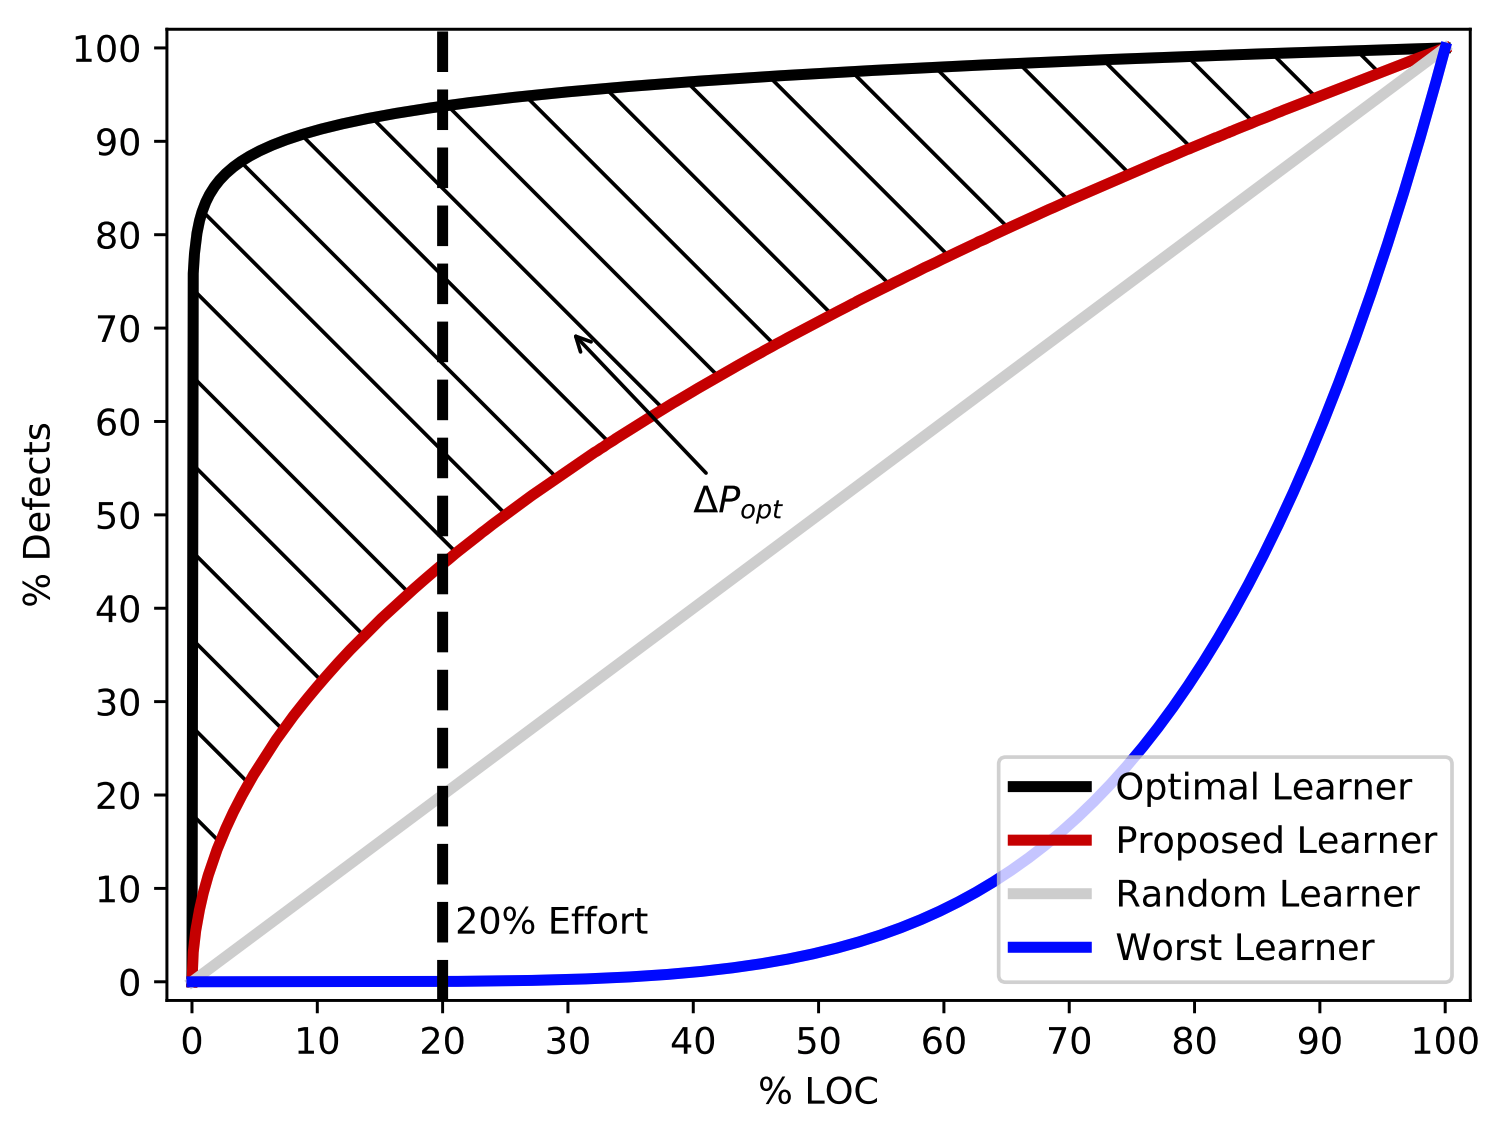
\includegraphics[width=2.5in]{popt.png} 
% \end{center}
% \caption{Calculating $P_{\mathit{opt}}$.}\label{fig:popt} 
% \end{figure} 
% To apply the 20:80 rule, our $E_2$ $P_{\mathit{opt}}$ 
% criteria reports what percent of the commits
% have been found after reading just $m$\% of the corpus.
% To computer this measure, we
% separated the commit messages into two lists:
% those that are predicted to be buggy, and the rest.
% Each list is then sorted on ascending order of size of the commit message. The sorted lists are then appended together, buggy first. By running over that list up to the $m$\% point (of lines of commit messages), we can report
% which is what percent of the buggy commits are found after
% reading just $m$\% of the commit messages. 
% $P_{\mathit{opt}}$ is defined as $1 - \Delta_{\mathit{opt}}$ with $\Delta_{opt}$ as the area between the effort cumulative lift charts of the optimal model (where we predict using the actual labels) and the prediction model (learned from a classifier).
% As shown in Figure \ref{fig:popt}, the x-axis is the
% percentage of required effort to inspect the commits and the y-axis is
% the percentage of buggy commits found in the selected code. 
% As the the ``worst'' model, that is learned by sorted
% the two lists {\em descending} on size of commits, with the buggy commit list explored last. 
% If 
% $S(\mathit{optimal}), S(m)$ and $S(\mathit{worst})$ are the area of curve
% under the optimal model, predicted model, and worst model
% up to some x-value of $m$,  then $P_{\mathit{opt}}(m)$ is:

% {\small \begin{equation}\label{eq:popt}
%  \mathit{E_2} = \mathit{P_{\mathit{opt}}(m)} = 1 - \frac{S(\mathit{optimal}) - S(m)}{S(\mathit{optimal}) - S(\mathit{worst})}
% \end{equation}}

\subsection{Statistical Methods}\label{tion:stats}

This study ranks treatments using the Scott-Knott procedure recommended by Mittas \& Angelis in their 2013 IEEE TSE paper~\cite{mittas2013ranking}. This method
sorts results from different treatments, then splits them in order to maximize the expected value of differences  in the observed performances
before and after divisions. For lists $l,m,n$ of size $\mathit{ls},\mathit{ms},\mathit{ns}$ where $l=m\cup n$, the ``best'' division maximizes $E(\Delta)$; i.e. the delta in the expected mean value before and after the spit: 

 \[E(\Delta)=\frac{ms}{ls}abs(m.\mu - l.\mu)^2 + \frac{ns}{ls}abs(n.\mu - l.\mu)^2\]

Scott-Knott then checks if that ``best'' division is actually useful. To implement that check, Scott-Knott would apply some statistical hypothesis test $H$ to check if $m,n$ are significantly different (and if so, Scott-Knott then recurses on each half of the ``best'' division). For this study, our hypothesis test $H$ was a conjunction of the A12 effect size test of and non-parametric bootstrap sampling; i.e. our Scott-Knott divided the data if {\em both} bootstrapping and an effect size test agreed that
the division was statistically significant (95\% confidence) and not a ``small'' effect ($A12 \ge 0.6$).

For a justification of the use of non-parametric bootstrapping, see Efron \& Tibshirani~\cite[p220-223]{efron94}. For a justification of the use of effect size tests see Kampenes~\cite{kampenes2007} who  warn that even if an hypothesis test declares two populations to be ``significantly'' different, then that result is misleading if the ``effect size'' is very small. Hence, to assess the performance differences  we first must rule out small effects. Vargha and Delaney's non-parametric $A12$ effect size test was endorsed by Arcuri and Briand~\cite{arcuri2011practical}.
This test 
explores two lists $M$ and $N$ of size $m$ and $n$ by computing the probability that numbers in one sample are bigger than in another as below:

\[
    A12 = \left(\sum_{x\in M, y \in N} \begin{array}{lr}
        1, & \mathit{if } x > y\\
        0.5, & \mathit{if } x == y
        \end{array}\right) / (mn)
\]



\subsection{Learners Used in this Study}\label{tion:learners}
There are very many ways to build a defect predictor.
This paper
uses methods that are (a)~standard in the literature as well as some that
have (b)~recently shown much promise.
For a definition of ``standard in the literature'', we use the Ghotra et al.
ICSE paper that grouped 32 defect predictors into different ranks
(see Table 9 of~\cite{ghotra15}). For this study we used Random Forests+J48  and Logistic Regression (which are two top-ranked 
learners, according to the Ghotra results).
Also, 
 just for completeness, we use Support Vector Machines (which comes from their bottom rank).
For the other learners, we use  one methods reported very recently at FSE'19 
(FFTs, describe below) as well as a standard data imbalance correction
algorithm called SMOTE.

\subsubsection{Logistic Regression (LR)}
Given a  regression function $t$
      that combines many variables, Linear Regresion (LR) maps $t$ into the range 0..1 using $u=1/(1+e^{-t})$~\cite{Witten:2011}. A binary classifier for class labels $x,y$ is then constructed using (e.g.)
 $\mathit{if}\; u<0.5\; \mathit{then}\; x\; \mathit{else}\;y$.
        
\subsubsection{Tree Learners: J48 + Random Forests (RF)}
J48  recursively builds one decision tree by
finding the feature whose ranges most reduce {\em entropy} (which is a measure of the division of class labels that call into each range).
 Using J48 as a sub-routine, our
 Random Forests   builds many trees,
 each time using  different  subsets of
 the  data rows $R$ and columns $C$\footnote{Specifically, using $\log_2{C}$ of the columns, selected at random.}. 
Test data is then passed across all $N$ trees and the conclusions are determined (say) a majority vote across all the trees~\cite{Breiman2001}. 

\subsubsection{Support Vector Machines (SVMs)}
SVMs created a hyperplane that maximize the distance between the two classes to it to separate them (i.e., defective or not). 
        In this paper, following the results of Ghotra et al. \cite{ghotra15}, the Sequential Minimal Optimization
        (SMO) SVM technique is used. SMO analytically solves the large
        Quadratic Programming (QP) optimization problem which
        occurs in SVM training by dividing the problem into a series
        of possible QP problems~\cite{zeng2008fast}.

\subsubsection{SMOTE}
        SMOTE is not a learner, but a data pre-processor.
        Given some data set where the number of positive and negative examples are not equal, SMOTE randomly discards members of the majority class while also creating synthetic examples of the minority class.
        For that creation, each row $x$ finds $y_1,..,y_5$ similar rows
        of the same class. It then picks of those rows 
        $y_i$ at random
        and creates a new example at a random selected distance between $x$ and $y_i$.  Some recent results report that off-the-shelf SMOTE can be improved by some local tuning~\cite{agrawal2018better,bennin2018mahakil}.
We do not use such local tuning since recently is has been shown that such tunings
are out-performed by FFTs (see below).

\subsubsection{Fast and Frugal Trees (FFTs)}
 All the   learners listed above execute in the same
        manner, no matter what   evaluation criteria  is used to assess their learned models.
        FFTs, on the other hand, change their reasoning based
        on the target evaluation ctieria. 
        
        More specifically, in this study,
        FFTs change  they way they rank numeric ranges according to the evaluation criteria. 
Specifically:
\bi
\item All numeric columns are divided at their medium values.
\item Each division is that  sorted by the predicated goal, sorted best to worst (if the goal is changed, FFTs would change how it sorts the  discretized ranges).  For both goals, the evaluation criteria scores {\em higher} if {\em more} bugs are found.
\ei
%(Note that if we changed the evaluation criteria, FFTs would then also change how it sorts the  discretized ranges.)

This sort order is used as follows.
 An FFTs is a decision tree made for binary tree where all internal nodes
have one leaf node with a guard condition leading to a classification decision~\cite{martignon2008categorization}.  Each leaf can have two  guards; specifically either the range associated with least or most $E_i$. This means  that,
for depth $d$, we build    $2^d$ trees.
For example, for d=4, \fig{fft} shows  one of the $2^d=16$ possible trees.
\begin{figure}
{\small
\begin{alltt}
    if          LA   \(<\)   10     then nonBuggy   
    else if     Entropy \(\le\) 0.65  then Buggy    
    else if     NS \(>\) 3          then Buggy   
    else if     FIX == 1        \hspace{0.02in}then Buggy    
    else                        \hspace{0.02in}nonBuggy        
\end{alltt}}
\caption{An FFTs tree. Built using the features of \tbl{metrics}.
The first guard of that tree is  {\em LA $<$ 10}  where this predicts for a nonBuggy commit. If that guard is false, then the reasoning falls down to the rest of the tree.
}\label{fig:fft}
\end{figure}
FFTs builds all 16 trees then sorts then  using the G-score  (by running  the training data through each one). The best tree (as discovered on the training data) is then applied to the test data.



Despite the apparent simplicity of  FFTs, Chen et al.~\cite{di18_fft}
reported that this method performs dramatically
better than many prior results
seen at recent ICSE conferences~\cite{ghotra15,agrawal2018better}.
(including those that used hyperparamter optimization
and data pre-processing with SMOTE). 
There are two possible
explanations for this superior performance. Firstly, due to their discretization policy, they can make better use of the evaluation criteria than any other learner (that builds
their models without reflecting over  the evaluation criteria). Secondly, the FFTs training process (of selecting the best out of 16 possible models) is essentially an ensemble
learning algorithm (albeit a very simple one) and such algorithms have been known to perform better than solo learners~\cite{kocaguneli2012value}.


%Despite the simplicity of the approach, FFTs  out-performs prior state-of-art results~\cite{di18_fft} in both classification and hyperparamter optimization results seen for defect prediction papers at recent ICSE conferences~\cite{ghotra15,agrawal2018better}. We have two explanations for this superior performance. Firstly, due to their discretization policy, they can make better use of the evaluation criteria than any other learner that builds their models without reflecting over  the evalaution criteria. Secondly, the FFTs training process (of selecting the best out of 16 possible models) is essentially an ensemble learning algorithm (albeit a very simple one) and such algorithms have been known to perform better than  solo learners.
 

% \bi
% \item PCMSolver (PCMSOLVER): An API for the Polarizable Continuum Model \cite{pcmsolver}.
% \item Xenon: A middleware abstraction library that provides a simple programming interface to various compute and storage resources \cite{xenon}.

% \item MDAnalysis (MDANALYSIS): a Python library to analyze molecular dynamics trajectories generated by a wide range of popular simulation packages \cite{mdanalysis}.
% \item HOOMD-blue (HOOMD): a general purpose particle simulation toolkit. It performs hard particle Monte Carlo simulations of a variety of shape classes, and molecular dynamics simulations of particles with a range of pair, bond, angle, and other potentials \cite{hoomd}.  
% \item ABINIT (ABINIT): an atomic-scale simulation software suite \cite{Abinit}.
% \item Amber (AMBER): Fast, parallelized molecular dynamics trajectory data analysis \cite{Amber-MD}.

% \item RMG-py (RMG-PY): Python version of Reaction Mechanism Generator, a tool for automatically generating chemical reaction mechanisms for modeling reaction systems including pyrolysis, combustion, atmospheric science, and more \cite{ReactionMechanismGenerator}.
% \item LAMMPS (LAMMPS): Large-scale Atomic/Molecular Massively Parallel Simulator, a classical molecular dynamics simulation code \cite{lammps-sandia}.
% \item libMesh (LIBMESH): a framework for the numerical simulation of partial differential equations using arbitrary unstructured discretizations on serial and parallel platforms. A major goal of the library is to provide support for adaptive mesh refinement (AMR) computations in parallel while allowing a research scientist to focus on the physics they are modeling \cite{libMesh}.
% \ei



 
 
% \begin{figure*}[!b]
% \small 
% \caption{RQ2  results - Median G-scores seen when learning on release $r$ and testing on release $r+1$ when the learner is FFTs
% and the labeling method is either keywords or FASTREAD. 
% As shown in \tbl{data}c, 
% different projects have different numbers of releases. Hence, in this figure, some of the projects have more results that the other.
%  In this figure, when two marks are not seen at the same x-value (e.g. PCMSOLVER), then one dot is obscuring the other.
% } 
% 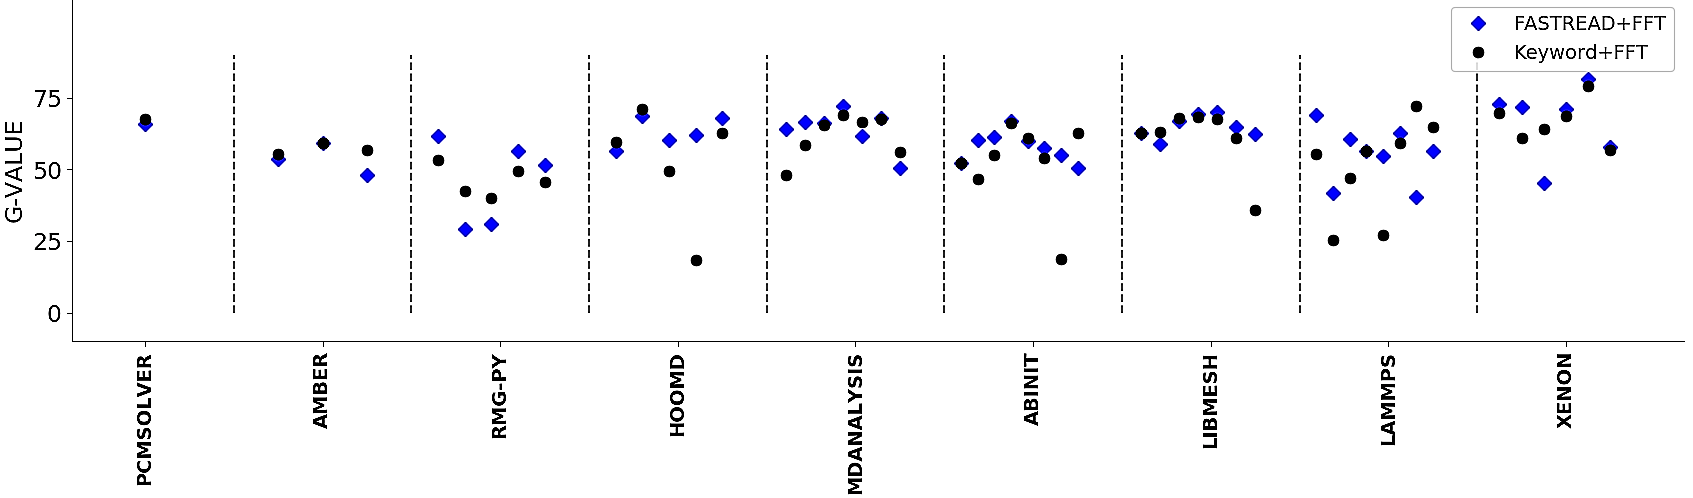
\includegraphics[width=\linewidth, height=1.8in]{rq2_1.png}
% \label{fig:rq2} 
% \end{figure*}
% % \begin{figure*}[!t]
% % \small
% % 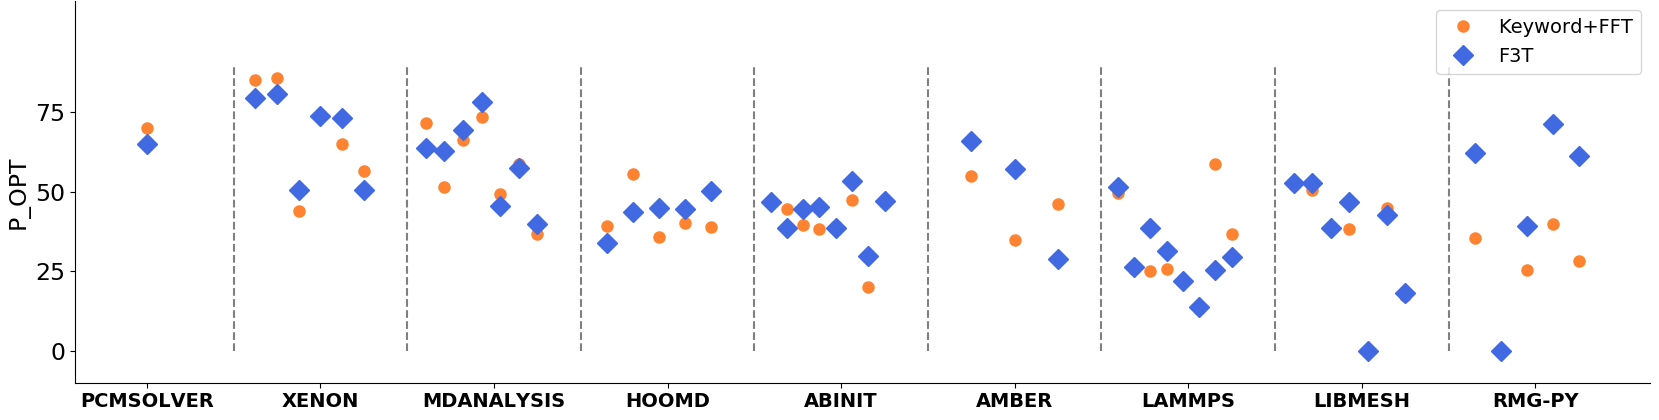
\includegraphics[width=\linewidth]{rq2_2.png}
% % \vspace{-20pt}
% % \end{figure*}


\subsection{Experimental Rig}\label{tion:eval}
For this study, it is important to test on data not used in training (to avoids overfitting on the training and inappropriately inflating the test performance scores). To that end, we
exploited the  the software release structure of our projects. Specifically, if a project had $R$
releases, then our learners were trained on release $r$ and tested on release $r+1$.

\subsection{Ground Truth}

For this study to work, some ``ground truth'' must be accessed against which we can compared different methods for labeling commit messages and classification. That ground truth was generated as follows.

Using pizza, we attracted half a dozen graduate students (computer science doctoral candidates) to spend a day labeling  commit messages. Messages were labelled ``buggy'' or ``not buggy''
at a rate of 8 messages/minutes/person. If this seems fast, then
note that the median size of these commit messages is not large. All the messages of \tbl{sample}
fall within the 25 to 75th percentile of commit message size. As a sanity check,  half of the labels were read by a second person. The observed disagreement rate was very low (under 15\%). 


\begin{table}[!t]
\caption{ Labels generated by FASTREAD text classifier for 100 randomly selected commits.  Scored via manual cross- inspection.
}\label{tbl:100}

\begin{center}
%\begin{threeparttable}
%\vspace{-10pt}
%\resizebox{!}{0.2\linewidth}{
%\setlength        abcolsep{10pt}
\begin{tabular}{ r|P{1.5cm}|P{1.8cm}}
 \multicolumn{1}{c|}{} & \multicolumn{1}{c|}{} & \multicolumn{1}{c}{False-Alarm}\\
 \multicolumn{1}{c|}{Dataset} & \multicolumn{1}{c|}{Recall} & \multicolumn{1}{c}{Rate}\\
\hline
PCMSOLVER & 72 & 21 \\
XENON & 96 & 21 \\
AMBER & 96 & 16 \\
HOOMD & 98 & 13 \\
RMG-PY & 89 &  3 \\
\end{tabular}
%}
%\end{threeparttable}
\end{center}
\end{table}

At the end of the labeling session,
only 16,000 commits from  four projects (out of a total of nine) had been labelled manually by human beings. The authors
of this paper considered reading on to manually label the remaining 29,000 commits from our other
five projects. But given the tedium of that  process,
 this was conjectured to introduce errors into our 
labels. Moreover, such manual methods are not appreciated in the industry. Hence, we tested if a faster semi-automatic method (i.e. FASTREAD) would suffice by investigating 100 of those labels (selected at random) from the rest five projects. These are manually cross-labeled 
to generate Table \ref{tbl:100}.
Note that our FASTREAD generated labels  
performed very well.

% {\setlength{\extrarowheight}{3.5pt} \begin{table}
% \small

% \caption{Evaluation Rigs for Research Questions}
% \label{tbl:rigs}
 
% \begin{center}
% %\begin{threeparttable}
% %\vspace{-10pt}
% %\resizebox{!}{0.2\linewidth}{
% %\setlength        abcolsep{10pt}
% \begin{tabular}{l|c|P{1.5cm}|P{1.5cm}|}
%  \multicolumn{1}{c}{} & &  \multicolumn{2}{|c|}{DATA MINING}\\
%  \multicolumn{1}{c}{} & &  \multicolumn{2}{|c|}{METHODS}\\
% \cline{3-4}
%  \multicolumn{1}{c}{} & & Traditional &  FFTs \\
% \hline
% \multicolumn{1}{c|}{labeling} & keywords & {\large I} & {\large III} \\ \cline{2-4}
% \multicolumn{1}{c|}{METHODS} & FASTREAD & {\large II} & {\large IV} \\ \hline
% \end{tabular}
% %}
% %\end{threeparttable}
% \end{center}
% \label{tbl:research}
% \end{table}




%Using  an SVM text classifier trained from the first four projects, we automatically labelled the commit messages in the remaining five projects. 



All this data was used as follows. In {\bf RQ1}, different labelling methods are compared to 
the ground truths (i.e. human labels) from the original four projects. During defect prediction of other
research questions ({\bf RQ2},{\bf RQ3}, and {\bf RQ4}), the human labels are utilized as the ground truths for
the original four projects. However, for the rest five projects,  $p_{i+1}[keyword]$ and $p_{i+1}[FASTREAD]$ are served as the ground truths for $p_{i}[keyword]$ and $p_{i}[FASTREAD]$ ($p_i$ - project at version i). It method is applied and endorsed through previous studies that solely using automating keyword  \cite{nayrolles18_clever, commitguru, kamei12_jit, catolino17_jitmobile}. 


% \begin{figure*}[!t]
% \caption{RQ3 numerical results. Traditional system versus $F^3T$ system (FASTREAD+FFT). In this figure, the {\em higher} the vertical bars, the {\em better} $F^3T$ performed  compared to  another learning method. Let $X$ be the $F^3T$ score and $Y$ is
% the score from another data mining method, then on this chart, the height of each bar is  median $X-Y$ seen across all tests in a project.}
% \begin{center}
% 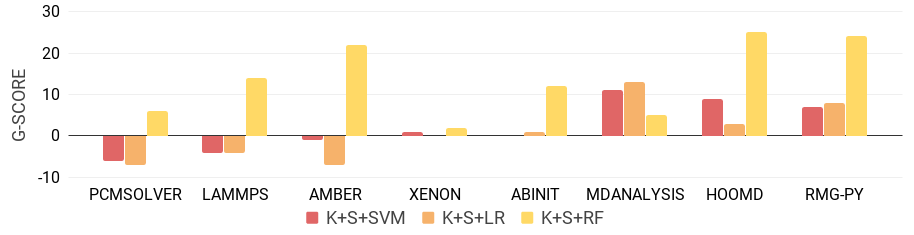
\includegraphics[width=5.5in]{rq4_final.png}
% \end{center}
% \label{fig:rq3} 
% \end{figure*}
\begin{table}[!t]
\caption{RQ1 results. Comparing FASTREAD (from $F^3T$) vs Keywords (from Commit.Guru) for worrying commits identification performance by comparing generated labels against  ``ground truth''; i.e. those
labels  assigned by human readers.}
\label{tbl:rq1}
 
\begin{center}
%\begin{threeparttable}
%\vspace{-10pt}
%\resizebox{!}{0.2\linewidth}{
%\setlength        abcolsep{10pt}

\begin{tabular}{ r|P{1.1cm}|P{1.35cm}|P{1.1cm}|P{1.25cm}}
\multicolumn{1}{c|}{} & \multicolumn{2}{c|}{} & \multicolumn{2}{c}{False-Alarm}\\
 \multicolumn{1}{c|}{} & \multicolumn{2}{c|}{Recall} & \multicolumn{2}{c}{Rate}\\
\cline{2-5}
 Dataset & Keyword & FASTREAD & Keyword & FASTREAD \\
\hline
LIBMESH & 74 & 97 & 24 & 17 \\
ABINIT  &  81 & 96 & 29 & 18 \\
MDANALYSIS   & 84 & 95 & 42 & 23 \\
LAMMPS   & 81 & 99 & 73 & 35 \\
\end{tabular}
%}
%\end{threeparttable}
\end{center}
\end{table}

 
\section{Results}
%Our research questions are designed so that it compares the combination of labeling methods and data mining methods from I to IV of traditional system to our proposed $F^3T$ system. RQ1 concerns the labeling quality so it compares II and IV, RQ2 concerns the data miner quality so it compares III and IV, and RQ3 focuses on the whole system so it compares I and IV.  \\

{\bf RQ1: How close are FASTREAD and keyword labeling to human labels?}

%Software maintenance is a continuing process, and software developers have the domain expertise in understanding the commit logs. 25,000+ commits are crossed labeled by SE Ph.D. students from 4 projects. With the initial assumption that software maintenance requires the expert's understanding, these human-labeled commit logs data from those four initial sampled repositories serves as the ground truth to compare the effectiveness of automatic Keywords versus FASTREAD tagging. FASTREAD statistically significant won across four cases with evaluation of recall and false-alarms (up to 23\% recall and 38\% false-alarm).  
This question compares  different labeling methods (keywords, FASTREAD)
against  ground truth labels (assigned by a team of humans).



In Table \ref{tbl:rq1},
labels generated by humans are used to score  labels proposed by FASTREAD or keywords. Note that keywords result in lower recall and higher false alarms; i.e.:
 

\begin{RQ}{\normalsize{Compared to humans...}} 
FASTREAD was best at reproducing the ground truth (i.e. the human labels).
\end{RQ}
 
 


\begin{table}[!b]
\caption{RQ2 results. Win percentages of G-score (left) and $P_{opt}(20)$ (right). Gray cells highlight the labelling method that were top-ranked most in that project by the statistical tests of \tion{stats}. 
Each cell is in the format of $P (W/N)$ where W is the number of times one treatment won over the other, and N is the number of the releases per project, then
the percentage win P is calculated by $W/N$. Treatments: Keyword+FFTs (K) and FASTREAD+FFTs (F)}
\label{tbl:rq2aaa}

\small 

\resizebox{\linewidth}{!}{
\hspace{-10pt}\begin{minipage}{0.54\linewidth}
\begin{tabular}{r@{~}|r@{~}|r@{~}}
\multicolumn{1}{c|}{} & \multicolumn{2}{c}{\textbf{\% G-score Wins}} \\
\cline{2-3}
\begin{tabular}[c]{@{}c@{}} \textbf{Dataset} \end{tabular} & 
\multicolumn{1}{c|}{\textbf{K}} & \multicolumn{1}{c}{\textbf{F}} \\ \hline
PCMSOLVER &  \cellcolor{gray!20} 100 (1/1) & 0 (0/1) \\ 
AMBER &  \cellcolor{gray!20} 67 (2/3) & 33 (1/3) \\ 
HOOMD & 40 (2/5) &  \cellcolor{gray!20} 60 (3/5)\\ 
RMG-PY  & 40 (2/5) &  \cellcolor{gray!20} 60 (3/5)\\ 
ABINIT & 25 (2/8) &  \cellcolor{gray!20} 63 (5/8) \\ 
LIBMESH & 28 (2/7) &  \cellcolor{gray!20} 72 (5/7)  \\  
MDANALYSIS & 28 (2/7) &  \cellcolor{gray!20} 72 (5/7) \\ 
LAMMPS & 25 (2/8) &  \cellcolor{gray!20} 75 (6/8)\\
XENON & 17 (1/6) &  \cellcolor{gray!20} 83 (5/6)  
\\  
\end{tabular}  %
\end{minipage} \
\hspace{25pt}\begin{minipage}{0.60\linewidth}
%\centering

\begin{tabular}{r@{~}|r@{~}|r@{~}}
\multicolumn{1}{c|}{} & \multicolumn{2}{c}{\textbf{\% $P_{opt}(20)$ Wins}} \\
\cline{2-3}
\begin{tabular}[c]{@{}c@{}} 
\textbf{Dataset} \end{tabular} & \multicolumn{1}{c|}{\textbf{K}} & \multicolumn{1}{c}{\textbf{F}} \\ \hline
PCMSOLVER &  \cellcolor{gray!20} 100(1/1) & 0(0/1) \\ 
XENON &  \cellcolor{gray!20} 50(3/6) &  \cellcolor{gray!20} 50(3/6)\\
MDANALYSIS & 43 (3/7) &  \cellcolor{gray!20} 57 (4/7)\\ 
LIBMESH & 14 (1/7) &  \cellcolor{gray!20} 57 (4/7)\\  
HOOMD & 40 (2/5) &  \cellcolor{gray!20} 60 (3/5)\\ 
LAMMPS & 25 (2/8) &  \cellcolor{gray!20} 63 (5/8)\\
ABINIT & 25 (2/8) &   \cellcolor{gray!20} 63 (5/8)\\
AMBER & 33 (1/3) &  \cellcolor{gray!20}  67 (2/3)\\
RMG-PY & 0 (0/5) &  \cellcolor{gray!20}  80 (4/5)
\\
\end{tabular}
\end{minipage}}
%\end{center} 
\vspace{-10pt}
\end{table}

%\end{center}  







\textbf{RQ2: Does keyword labeling lead to  better predictors for buggy commits?}

 {\bf RQ1} only explored  labeling.  
In {\bf RQ2}, we 
check how well those labels predict for defects.
For this research question, we kept the learner constant  (only FFTs) and varied
the labeling method (keywords or FASTREAD).
  
From labels for buggy and non-buggy commits, we applied
the SZZ algorithm from Commit.Guru to  find which code commits that lead to bugs.
All such code is labelled ``buggy=yes'' and all other code is labelled ``buggy=no''.

Table \ref{tbl:rq2aaa} compares predictive performance using FFT+FASTREAD (i.e. $F^3T$) and
FFT+standard keyword labeling (using Commit.Guru). Gray cells denote treatments with superior performance.
 Note that, in the majority case (7 out of 9 projects for both G-score and $P_{opt}(20)$),  $F^3T$ performs best.  That is:
% with another lear

% back to find bug-inducing code changes. 


% that introducing defects to the software. Each of these commits will be analyzed and recommended metrics are extracted to describe how buggy each commit is. 
% Finding the right bug-inducing commits will help to link to the right bug-inducing commits with appropriate values of metrics to build a strong model to predict future buggy software commits. Our recommended data mining method is FFTs with no pre-processing. 

% From two ways to label the issues (keywords or FASTREAD), data are curated and built by the FFTs learner.  Table \ref{tb:rq2} recorded the percentage of statistically significant winning or ranking higher across all the releases in each project. 
% Specifically, for LAMMPS, there are 9 releases, so the performance metrics are collected 8 times incrementally and FFTs model built on FASTREAD generated data won 6/8 for G-score so $F^3T$ won 75\% time for G-score. The higher number between the twos is the better combination method which is indicated by the highlighted cell for each project row. With 7 wins out of 9 projects for G-score, FFTs model built on FASTREAD generated data outperformed FFTs model built on Keyword generated data. Hence,
%Essentially, Figure \ref{fig:rq2} shows results where one learner (FFTs) uses two different ways to label the issues (keywords or FASTREAD). In figure \ref{fig:rq2},  each y-axis value shows the performance at the median difference of the two methods between all the releases per project. Note that in this figure, the keyword and FASTREAD results for the same test set are directly above/below each other. The \textbf{\color[rgb]{1, 0.39, 0.28} orange} diamond represents FASTREAD+FFTs (i.e $F^3T$) while the \textbf{\color{yellow} yellow}  circle represents Keyword+FFTs. The quality of the data from our proposed method can be easily spotted at the last five projects of each figure and similar performance on the rest (except K+FFTs performed worse on $P_{opt}(20)$ in PCMSOLVER).  


%In that a figure,  Each x-axis value shows different test results when release $r-1$ was used to train a classifier and release $r$ was used to test that classifier. Note that in this figure, the keyword and FASTREAD results for the same test set are directly above/below each other. The \textbf{\color{blue} blue} diamond represents $F^3T$ while the \textbf{\color{orange} orange}  circle represents Keyword+FFTs. A lot of the differences between the two methods are easy to spot (i.e. performance on $P_{opt}(20)$ chart for RMG-PY), but some are not (i.e. performance on G-score chart for AMBER). 




%In the 50 results of \fig{rq2} there are only 13 results on for each criterias, G-score and $P_{opt}(20)$, where keywords generated data lead to a higher performance of the model. Further, within each of the nine projects, there are zero and only 2 cases for G-score and $P_{opt}(20)$ respectively where keywords usually performed best (where ``usually'' is defined to mean ``in half the releases or more'').




%Four initial datasets that got human ground truth labels are expressed in highlighted entries. W
 
 %Four popular repositories that satisfy our sanity checks were picked at random, and their commit logs were sampled to be labeled for buggy commits by a human. 


\begin{RQ}{\normalsize{Compared to keywords labeling...}} 
FASTREAD’s generated better predictors for buggy code. 
\end{RQ}



% \begin{table}[!t]
% \small
% \begin{center}
% \caption{RQ2 Statistical Result - G-score percentage performance comparison of statistically significant wins across all the releases per project between FASTREAD+FFTs ($F^3T$) versus Keyword+FFT(K+FFT)}
% \label{tbl:rq2}

% \hspace{-15pt}\resizebox{1.02\linewidth}{!}{ \begin{tabular}{c@{~}|r@{~}|r@{~}|r@{~}|r@{~}}
% \multicolumn{1}{c|}{} & \multicolumn{4}{c}{\textbf{\% G-score Wins}} \\
% \cline{2-5}
% \begin{tabular}[c]{@{}c@{}} \textbf{Dataset} \end{tabular} & \begin{tabular}[c]{@{}c@{}} \textbf{SMOTE+RF}\end{tabular} & \textbf{SMOTE+SVM} & \begin{tabular}[c]{@{}c@{}} \textbf{SMOTE+LR}\end{tabular} & \textbf{FFTs} \\ \hline
% AMBER & \cellcolor{gray!20} 67 (2/3) & 0 (0/3) & 0 (0/3) & 0 (0/3) \\ 
% PCMSOLVER & 0 (0/1) & 0 (0/1) & \cellcolor{gray!20} 100 (1/1) & 0 (0/1) \\ 
% RMG-PY & 0 (0/5) & 0 (0/5) & \cellcolor{gray!20} 40 (2/5) & 0 (0/5) \\ 
%  HOOMD & 0 (0/5) & 0 (0/5) & 0 (0/5) & \cellcolor{gray!20} 40 (2/5)  \\ 
%  LAMMPS & 0 (1/8) & 13 (1/8) & 0 (0/8) & \cellcolor{gray!20} 50 (4/8)  \\  
%  ABINIT & 0 (0/8) & 0 (0/8) & 13 (1/8) & \cellcolor{gray!20} 50 (4/8) \\
%  XENON & 17 (1/6) & 0 (0/6) & 17 (1/6) & \cellcolor{gray!20} 50 (3/6) \\ 
% MDANALYSIS & 0 (0/7) & 0 (0/7) & 0 (0/7) & \cellcolor{gray!20} 72 (6/7) \\ 
% LIBMESH & 0 (0/7) & 0 (0/7) & 0 (0/7) & \cellcolor{gray!20} 100 (7/7) \\ 
% \end{tabular}}
% \end{center} 
% \vspace{-10pt}
% \end{table} 
 
%\fig{rq2} shows results where one learner (FFT) uses two different ways to label the issues (keywords or FASTREAD).  In that a figure,  Each x-axis value shows different test results when release $r-1$ was used to train a classifier and release $r$ was used to test that classifier.  Note that in this figure, the keyword and FASTREAD results for the same test set are directly above/below each other.

%In the 50 results of \fig{rq2}, there are only nine results where  keywords lead to a higher G-score than FASTREAD. Further, within each of the nine projects, there are zero cases where keywords usually performed best (where ``usually'' is defined to mean ``in half the releases or more''). Hence, we say:


%\begin{RQ}{Compared to keyword labeling...} 
%FASTREAD's   generated better   predictors for buggy commit messages.
%\end{RQ}
  

%  \begin{table}[!t]
% \footnotesize
% \begin{center}
% \caption{RQ2 results: FFTs Validation Statistical Results - G-score (top) and $P_{\mathit{opt}}$ (bottom) percentage performance comparison of statistically significant wins across all the releases per project between FFTs versus state-of-the-art methods (SMOTE+SVM, SMOTE+RF, and SMOTE+LR)}
% \label{tbl:rq4}
% \begin{tabular}{c@{~}|r@{~}|r@{~}|r@{~}|r@{~}}
% \multicolumn{1}{c|}{} & \multicolumn{4}{c}{        \textbf{\% G-score Wins}} \\
% \cline{2-5}
% \begin{tabular}[c]{@{}c@{}}         \textbf{Dataset} \end{tabular} & \begin{tabular}[c]{@{}c@{}}         \textbf{SMOTE+RF}\end{tabular} &         \textbf{SMOTE+SVM} & \begin{tabular}[c]{@{}c@{}}         \textbf{SMOTE+LR}\end{tabular} &         \textbf{FFT} \\ \hline
% PCMSOLVER & 0 & 0 & 100 & 0  \\ 
% AMBER & 0 & 0 & 33 & 33  \\ 
% LAMMPS & 0 & 0 & 0 & 37  \\  
% XENON & 0 & 0 & 16 & 50 \\ 
% ABINIT & 0 & 0 & 12 & 50  \\  
% HOOMD & 0 & 0 & 0 & 60\\ 
% RMG-PY & 0 & 0 & 0 & 60\\ 
% MDANALYSIS & 0 & 0 & 0 & 71\\ 
% LIBMESH & 0 & 0 & 0 & 100\\ 
% \end{tabular}
% \end{center} 
% \vspace{-10pt}
% \end{table} 

% {\bf RQ2: Which predicting method is best for buggy commits?}


% Based on the {\bf RQ1} results, we now deprecate keyword labeling. Now, in {\bf RQ2}, we assume labeling with FASTREAD and then ask  ``what predicting method leads to best results?''.   
 
% %Based on the {\bf RQ1} results, keyword labeling can be deprecated for a moment. labeling task comes prediction task.
% %Data is curated from FASTREAD labeling here to investigate the best data mining methods for commit-level defect prediction of computational software. 
 
% Table \ref{tbl:rq2} compares the performance of FFTs versus our other learning methods (standard miners with
%  data pre-processor SMOTE) building on FASTREAD generated data (rig IV versus rig II). Similar to \textit{RQ1.2}, we noted:
 
% \bi
% \item FFTs performs as well, or better, that the other learners in 6/9 projects for G-score comparisons.
% \item Traditional data mining methods mostly performs as well or better in a few projects (e.g. SMOTE+LR and SMOTE+RF won only 2 and 1 out of 9 projects). 

% %\item  When $F^3T$ performs comparatively  better, it can do so  by a large amount (often, more than 15\% better).
% %\item When $F^3T$ performs comparatively worse, the size of its loss is not large (evidence: see the left-hand-side negative vertical bars where $F^3T$ losses by just 3\% (median value).
% \ei

% The result is quite clear and we can conclude:


 
 

%  \fig{rq3} compares the performance of FASTREAD+FFTs versus our other learners (combined with the SMOTE
%  data pre-processor). In this chart, the more {\em higher} the bars, the {\em better} $F^3T$ performed
%  compared to other methods. 
% Note that:
% \bi
% \item   $F^3T$ performs as well, or better, that the other learners in 21/27 comparisons.
% \item $F^3T$ always performs much better than random forests (RF). 
% \item  When $F^3T$ performs comparatively  better, it can do so  by a large amount (often, more than 15\% better).
% \item When $F^3T$ performs comparatively worse, the size of its loss is not large (evidence: see the
% left-hand-side negative vertical bars where $F^3T$ losses by just 3\% (median value).
% \ei
% For completeness sake, we have conducted a non-parametric statistical test comparing the distribution
% of results seen in each project. A Cliffs-Delta and a Bootstrap  test  (at
% 95\% confidence) reports that  in all data sets, the $F^3T$ results are better than the other learners by more
% than a small effect and by a statistically significant amount. Hence we conclude that:

%\begin{RQ}{\normalsize{Compared to other predicting methods...}}
%FFTs performed best in classifying buggy commits.
%\end{RQ} 



{\bf RQ3:  What classifier  best predicts for buggy code?}

Recall that
{\bf RQ2} built predictors using only one classifier (FFTs). 
Now, for {\bf RQ3},  we used the labeling method endorsed
by {\bf RQ2} (FASTREAD) and varied
the data mining algorithm.
Using the rationale of 
\tion{learners},
{\bf RQ3} applied
FFTs, Logistic Regression, Random Forests,
Support Vector Machines, and the SMOTE preprocessor.


\tbl{rq3} shows those results.
As before, 
gray cells denote treatments with superior performance. FFTs performs as well or better in the majority cases (6/9 projects) for both G-score and $P_{opt}20$. That is:
 

\begin{RQ}{Compared to other predicting methods...} 
Of  the  predicting methods  studies  here,
FFTs built the best classifiers for buggy commits.
\end{RQ}

\begin{table}[!b]
\begin{center}
\caption{RQ3 results. Win percentages of G-score (top) and $P_{opt}(20)$ (bottom). 
 Gray cells highlight predicting methods that were top-ranked the most in that project
by the statistical tests of \tion{stats} (in $P(W/N)$ format).
(S= SMOTE, SVM= Support Vector Machine, RF= Random Forest,  LR= Logistic Regression)}
\label{tbl:rq3}
\footnotesize
\hspace{-8pt}\resizebox{1\linewidth}{!}{
\begin{tabular}{r@{~}|r@{~}|r@{~}|r@{~}|r@{~}}
\footnotesize
 & \multicolumn{4}{c}{\textbf{\% G-score Wins}} \\
\cline{2-5}
\begin{tabular}[c]{@{}c@{}} \textbf{Dataset} \end{tabular} & \begin{tabular}[c]{@{}c@{}} \textbf{SMOTE+RF}\end{tabular} & \textbf{SMOTE+SVM} & \begin{tabular}[c]{@{}c@{}} \textbf{SMOTE+LR}\end{tabular} & \textbf{FFTs} \\ \hline
AMBER & \cellcolor{gray!20} 67 (2/3) & 0 (0/3) & 0 (0/3) & 0 (0/3) \\ 
PCMSOLVER & 0 (0/1) & 0 (0/1) & \cellcolor{gray!20} 100 (1/1) & 0 (0/1) \\ 
RMG-PY & 0 (0/5) & 0 (0/5) & \cellcolor{gray!20} 40 (2/5) & 0 (0/5) \\ 
 HOOMD & 0 (0/5) & 0 (0/5) & 0 (0/5) & \cellcolor{gray!20} 40 (2/5)  \\ 
 LAMMPS & 0 (1/8) & 13 (1/8) & 0 (0/8) & \cellcolor{gray!20} 50 (4/8)  \\  
 ABINIT & 0 (0/8) & 0 (0/8) & 13 (1/8) & \cellcolor{gray!20} 50 (4/8) \\
 XENON & 17 (1/6) & 0 (0/6) & 17 (1/6) & \cellcolor{gray!20} 50 (3/6) \\ 
MDANALYSIS & 0 (0/7) & 0 (0/7) & 0 (0/7) & \cellcolor{gray!20} 72 (6/7) \\ 
LIBMESH & 0 (0/7) & 0 (0/7) & 0 (0/7) & \cellcolor{gray!20} 100 (7/7) \\
\end{tabular}}
\vspace{5mm}
\hspace{-8pt}\resizebox{\linewidth}{!}{ \begin{tabular}{r@{~}|r@{~}|r@{~}|r@{~}|r@{~}}
\multicolumn{1}{c|}{} & \multicolumn{4}{c}{\textbf{\% $P_{opt}(20)$ Wins}} \\
\cline{2-5}
\footnotesize
\begin{tabular}[c]{@{}c@{}} \textbf{Dataset} \end{tabular} & \begin{tabular}[c]{@{}c@{}}    \textbf{SMOTE+RF}\end{tabular} & \textbf{SMOTE+SVM} & \begin{tabular}[c]{@{}c@{}} \textbf{SMOTE+LR}\end{tabular} & \textbf{FFTs} \\ \hline
LAMMPS & \cellcolor{gray!20} 38 (3/8) & 13 (1/8) & 0 (0/8) & 0 (0/8)  \\  
XENON  & \cellcolor{gray!20} 33 (2/6) & 0 (0/6) & 17 (1/6) & 0 (0/6) \\ 
ABINIT & 0 (0/8) & \cellcolor{gray!20} 25 (2/8) & 0 (0/8) & 13 (1/8) \\ 
MDANALYSIS & \cellcolor{gray!20} 15 (1/7) & 0 (0/7) & 0 (0/7) & \cellcolor{gray!20} 15 (1/7) \\ 
AMBER  & 0 (0/3) & \cellcolor{gray!20} 33 (1/3) & 0 (0/3) & \cellcolor{gray!20} 33 (1/3) \\ 
HOOMD  & 20 (1/5) & 0 (0/5) & 0 (0/5) & \cellcolor{gray!20} 40 (2/5) \\ 
RMG-PY & 0 (0/5) & 0 (0/5) & 0 (0/5) & \cellcolor{gray!20} 40 (2/5) \\ 
LIBMESH & 15 (1/7) & 0 (0/7) & 0 (0/7) & \cellcolor{gray!20} 57 (4/7) \\ 
PCMSOLVER & 0 (0/1) & 0 (0/1) & 0 (0/1) & \cellcolor{gray!20} 100 (1/1) \\ 
\end{tabular}}
\end{center} 
\vspace{-10pt}
\end{table}

{\bf RQ4: Which identification and prediction system perform best for buggy commits?}


FASTREAD improves the dependent features quality or the correctness of buggy software commit identification, target for prediction task (from \textbf{RQ1} and \textbf{RQ2}) while FFTs model has proven to be a strong data miner for software analytics task (from \textbf{RQ3}). To complete the picture, for \textbf{RQ4},  our recommended $F^3T$ system from this paper is compared against state-of-the-art buggy software identification and prediction system, updated Commit.Guru (keywords labeling + traditional predicting methods). 

\tbl{rq4} shows those results.
As before, 
gray cells denote treatments with superior performance.
 Note that, in the majority case,  $F^3T$ performs as well or better (where most are better) than other systems in 8/9 for both G-score and $P_{opt}20$. Moreover, the higher win percentage across all the releases (e.g. for RMG-PY, $F^3T$ outperformed on 4 releases here while only on 2 releases in \textbf{RQ3}) and across projects (e.g. for $P_{opt}(20)$, $F^3T$ performs similarly or better in 6/9 projects for \textbf{RQ2} but 8/9 projects here) confirming the joint importance of data quality from FASTREAD labeling and FFTs for defect predicting. That is:

\begin{RQ}{Compared to the state-of-the-art system ...}

The proposed $F^3T$ outperformed the existing system buggy commits identification and prediction.

\end{RQ}



\begin{table}[!t]
\begin{center}
\caption{RQ4  results. Wins percentage of G-score (top) and $P_{opt}(20)$ (bottom). 
 Gray cells highlight bugs identification and prediction system  that were top-ranked
by the statistical tests of \tion{stats} (in $P(W/N)$ format).
$F^3T$= FFT+FASTREAD,
S= SMOTE. SVM= support vector machine. RF= Random Forest.  LR= Logistic Regression. K= keyword labeling
(with Commit.Guru). }
\label{tbl:rq4}
\scriptsize
\resizebox{0.95\linewidth}{!}{
 \begin{tabular}{r@{~}|r@{~}|r@{~}|r@{~}|r@{~}}
\multicolumn{1}{c|}{} & \multicolumn{4}{c}{\textbf{\% G-score Wins}} \\
\cline{2-5}
\begin{tabular}[c]{@{}c@{}} \textbf{Dataset} \end{tabular} & \begin{tabular}[c]{@{}c@{}} \textbf{K+S+RF}\end{tabular} & \textbf{K+S+SVM} & \begin{tabular}[c]{@{}c@{}} \textbf{K+S+LR}\end{tabular} & \textbf{$F^3T$} \\ \hline
PCMSOLVER & 0 (0/1) & 0 (0/1) & \cellcolor{gray!20} 100 (1/1) & 0 (0/1)  \\ 
AMBER & 0 (0/3) & 0 (0/3) & \cellcolor{gray!20} 33 (1/3) & \cellcolor{gray!20} 33 (1/3)  \\ 
LAMMPS & 0 (0/8) & 0 (0/8) & 0 (0/8) & \cellcolor{gray!20} 38 (3/8) \\  
ABINIT & 0 (0/8) & 0 (0/8) & 13 (1/8) & \cellcolor{gray!20} 50 (4/8) \\
XENON & 0 (0/6) & 0 (0/6) & 17 (1/6)& \cellcolor{gray!20} 50 (3/6)\\ 
HOOMD & 0 (0/5) & 0 (0/5) & 0 (0/5) & \cellcolor{gray!20} 60 (3/5)  \\ 
RMG-PY & 0 (0/5) & 0 (0/5) & 0 (0/5) & \cellcolor{gray!20} 60 (3/5) \\ 
MDANALYSIS & 0 (0/7) & 0 (0/7) & 0 (0/7) & \cellcolor{gray!20} 72 (5/7) \\ 
LIBMESH & 0 (0/7) & 0 (0/7) & 0 (0/7) & \cellcolor{gray!20} 100 (7/7) 
\\
\end{tabular}}
% 

\vspace{5mm}


\resizebox{0.95\linewidth}{!}{ \begin{tabular}{r@{~}|r@{~}|r@{~}|r@{~}|r@{~}}
\multicolumn{1}{c|}{} & \multicolumn{4}{c}{\textbf{\% $P_{opt}(20)$ Wins}} \\
\cline{2-5}
\begin{tabular}[c]{@{}c@{}} \textbf{Dataset} \end{tabular} & \begin{tabular}[c]{@{}c@{}}    \textbf{K+S+RF}\end{tabular} & \textbf{K+S+SVM} & \begin{tabular}[c]{@{}c@{}} \textbf{K+S+LR}\end{tabular} & \textbf{$F^3T$} \\ \hline
PCMSOLVER & \cellcolor{gray!20} 0 (0/1) & \cellcolor{gray!20} 0 (0/1) & \cellcolor{gray!20} 0 (0/1) & \cellcolor{gray!20} 0 (0/1) \\
LAMMPS & \cellcolor{gray!20} 38 (3/8) & 0 (0/8) & 0 (0/8) & 13 (1/8)  \\
MDANALYSIS & \cellcolor{gray!20} 29 (2/7) & 0 (0/7) & 0 (0/7) & \cellcolor{gray!20} 29 (2/7) \\
 HOOMD  & 0 (0/5) & 0 (0/5) & 0 (0/5) & \cellcolor{gray!20} 20 (1/5) \\ 
XENON  & 17 (1/6) & 0 (0/6) & 0 (0/6) &  \cellcolor{gray!20} 33 (2/6) \\ 
ABINIT & 0 (0/8) & 0 (0/8) & 0 (0/8) & \cellcolor{gray!20} 38 (3/8) \\ 
LIBMESH & 15 (1/7) & 0 (0/7) & 0 (0/7) & \cellcolor{gray!20} 57 (4/7) \\ 
AMBER  & 0 (0/5) & 33 (1/3) & 0 (0/3) & \cellcolor{gray!20} 67 (2/3) \\ 
RMG-PY & 0 (0/5) & 0 (0/5) & 0 (0/5) & \cellcolor{gray!20} 80 (4/5) 
\\
\end{tabular}}
\end{center} 
\vspace{-10pt}
\end{table}

\section{Discussion}\label{tion:time}


The statistical results of the last section do not
fully characterize the improvements achieved
by $F^3T$. For instance, \fig{rq3_1} visualizes the differencees
between the standard system (i.e. Commit.Guru) and $F^3T$ for our corpus.
Some of those improvements are very large indeed  (up to 48\% as the median absolute difference for G-score). For space reason, the improvements for both metrics from {\bf RQ3} can be accessed online \footnote{See github.com/sillywalk/defect-prediction/issues/20.}.   



 




Moreover, using the experience gained from the manual labeling from the above studies, we offer the observations
of Table \ref{tbl:time1} and \ref{tbl:time2}.
These tables  detail the time and cost required
to complete our work. Using this information, we can now
justify the calculations of \tion{iia}.
Recall that those calculations showed that for large
labeling tasks, the methods of this paper can reduce the
resources required for labeling by over an order of magnitude
(as seen in Table~\ref{tbl:time2}, from \$472K to just under \$38K).

That is to say, 
\fig{rq3_1}  and  Table~\ref{tbl:time2} show that for the corpus
studied here, active learning with FASTREAD plus the
FFTs (i.e. $F^3T$ learner lead to much better defect predictors,
generated using far less effort.




\section{Threats to Validity }

\subsection{Sampling Bias}

Like any data mining paper,
our work is threatened by  sampling bias; i.e.  what holds for the data we studied here may
not hold for other kinds of data. 
Within the space of one paper, it is hard to avoid sampling bias.
However, what researchers can do is make all their scripts and data available
such that other researchers can test their conclusions whenever new data becomes available. To that end, we ahve made all our scripts and data available at github.com/sillywalk/defect-prediction/.

\begin{table}[!t]
\vspace{-10pt}
\caption{Time cost model for manual versus FASTREAD labeling}
\vspace{-10pt}
\label{tbl:time1}
 
\begin{center}
%\begin{threeparttable}
%\vspace{-10pt}
%\resizebox{!}{0.2\linewidth}{
%\setlength        abcolsep{10pt}
\begin{tabular}{ l|c|c }
 \multicolumn{1}{c|}{} & \multicolumn{1}{c|}{Manual} & \multicolumn{1}{c}{FASTREAD}\\
\hline
time per commit & 8 secs & 4 secs \\
commits need to read & 5000 & 835 \\
time per project & 44.4 hours & 3.56 hours \\
\end{tabular}
%}
%\end{threeparttable}
\end{center}
\vspace{-1mm}
\end{table}

\begin{table}[!t]
\caption{Money cost model for manual versus FASTREAD labeling}
\label{tbl:time2}
\vspace{-10pt}
\begin{center}

%\begin{threeparttable}
%\vspace{-10pt}
%\resizebox{!}{0.2\linewidth}{
%\setlength        abcolsep{10pt}
\begin{tabular}{ l|c|c }
 \multicolumn{1}{c|}{} & \multicolumn{1}{c|}{Manual} & \multicolumn{1}{c}{FASTREAD}\\
\hline
commits per hour & 450 & 900 \\
money per hour & 9 & 18 \\
money per project & \$200 & \$32 \\
money for 590 projects & \$472,000 & \$37,760 \\ 
\end{tabular}
%}
%\end{threeparttable}
\end{center}
\vspace{2mm}
\end{table}
\subsection{Learner Bias}

This study compared our preferred methods to
 Logistic Regression, Random Forest, and Support Vector Machine (in the combination with SMOTE). 
 The case was made in \S 4.5 that this represents an interesting range of current practice.
 Nevertheless, it might be useful in future work to test if the central
claim of this paper (that a combination of human+artificial intelligence called FASTREAD is a good way to label commit messages)
hold across multiple classifiers.


\subsection{Evaluation Bias}

This paper employed  the G-score as defined in Equation 3.
This value is the harmonic mean between recall and false-alarm of risky software commit prediction power. There are other evaluation scores that could be applied to this kind of analysis~\cite{lo17_ifa}
and, in the future, it would be useful to test in the central claim of this paper holds for more than just G-scores and $P_{opt}(20)$.

% Note that we have already done those tests for one other evalaution method )the 20/80 rule proposed by Ostrand et al.).
% Those results are reported online \footnote{
%   See github.com/sillywalk/defect-prediction/issues/18,19,20.} . In summary, when assessed by that additional criteria, all our answers
% to {\bf RQ1,2,3,\& 4} remain the same.

% \subsection{Order Bias}

% For the performance evaluation part, the order that the data trained and predicted affects the results. XXX
% For this risky software commit prediction datasets, an ordering is deliberately chosen to mimic how a software is developed which leads to that our bias is required and needed. 
\section{Future Work}
As to future work, there are many options.
For example, 
we could repeat this study on more data.

Also,
we could explore other control parameters for FASTREAD.
All the above results were obtained using Yu et al.'s \cite{Yu:2018} original requirements (e.g. the values of  $\{N_1=1, N_2=30, N_3=95\%\}$) within the FASTREAD method. It is  is possible that other settings for these parameters could lead to better results.

Further,
all the work studied here relied on an off the-shelf  
 Sliwerski, Zimmermann, and Zeller's SZZ's
 algorithm~\cite{costa17szz, Kim08changes, Sliwerski05changes} (implemented through Commit.Guru)
 that traced back to the  bug inducing commits.
 SZZ itself is an algorithm under active research
 and there are numerous proposed improvements \cite{costa17szz}
 that could be useful for our work.

Another issue is that all the data-mining process in this paper  focused on learning the change level or commit-level as a whole. 
In this approach,
changes attributes on multiple files  (from Table \ref{tbl:metrics}) are averaged out within a commit \cite{kamei12_jit, commitguru, nayrolles18_clever, yan18_tddetermination}. This tend to be language agnostic and the results can be generalized. However, that approach might be enhanced
by including features extracted within the commit messages
(as proposed by Yan et al. \cite{yan18_tddetermination})
or by  including file or function attributes (i.e. learning on static code attributes such as C.K. and McGabe metrics) \cite{dpmetrics94, Fu2016TuningFS, danijel13lit, Jureczko10oodp, ghotra15, nagappan05, menzies07dp, menzies10dp, krishna16bellwether, nam18tse, agrawal2019dodge, di18_fft, Tu18Tuning, agrawal2018better} that are more granulated and high-dimensional.

Finally,
hyperparameter optimization technology keeps evolving.
 Agrawal et al. \cite{agrawal2019dodge} recently argued
 that for any dataset where FFTs are effective, that there is a better
 algorithm (that they call 
 $DODGE(\epsilon)$) which might be more effective.
 This is a promising avenue for future work.
 



\section{Conclusion}



From ``worrying'' or ``not worrying'' labelling, the bugs ground truth as a core for many analytics tasks is obtained.  
But different kinds of software use 
different language to describe their bugs. Hence, as shown in \fig{rq3_1}, standard labelling methods can  perform   badly 
when applied to new kinds
of software (e.g. the computational science projects explored here).

Intuitively, one way to find the labels is to create teams of humans to manually read all the commits. As details in \tion{iia}, that process can get very expensive.

Another way to find the labels is to use incremental AI tools that learn an
appropriate local model. Such  AI tools can present
examples to a human,  one  at a time. Whenever a human
offers a label to an example, the AI can update its internal model.
This internal model can be used to look ahead to find the next most-likely-to-be-worrying example.
After  a few loops of this process, the AI tool might be able to learn a model
that can find nearly all the remaining worrying commits. 


% The central insight of this paper is that commit labelingis  analogous  to  reading  research  papers  and  the  defectpredicting on commit level is analogous to traditional defectpredicting  on  release  level.  Hence,  an  active  learner  likeFASTREAD (designed for reading research papers) and FFTs(adapted from release-level defect prediction) could also beusefully  deployed  for  handling  buggy  commits  identifica-tion and prediction.



% This work introduced $F^3T$ system for software quality assurance when ingesting data from a version control system. It is a combination of (1) FASTREAD for buggy commits identification and (2) FFTs as the data miner:
% \bi
% \item
% FASTREAD is an active learner to achieve the human+artificial intelligence partnership to perform certain human-intensive parts of software analytics that is domain specialized (i.e. computational science software for our study). 
% \otem
% FFTs is an ensemble learner that have shown promises in recent works \cite{di18_fft}.    
% \ei
% %This paper has argued that a combination of human+artificial intelligence (the FASTREAD active learner) is a useful way to perform certain human-intensive parts of software analytics. Specifically, when ingesting data from a version control system, humans+AI form a  partnership where the AI roams over most of the data, bring back the most interesting examples for humans to review.

% The central insight of this paper is the importance of ground truths quality combining with the discriminative power of the right data miner. For commit labeling, the
% problem  is   analogous to reading research papers. Hence,
% the FASTREAD active learner, which was designed for reading research papers, could also be usefully deployed for handling commit messages. It is very important to obtain high quality labels,  such labels are the core requirement for a wide range of research tasks (for a long list of such tasks, see \S 2.4). Moreover, for prediction task, by choosing FFTs (i.e. the data miner with high discriminative power from literatures \cite{di18_fft} that was validated also in our studies) will result in the right conclusions for the analysis.  


%The central insight of this paper is that the commit labeling problem  is   analogous to reading research papers. Hence, the FASTREAD active learner, which was designed for    reading research papers, could also be usefully deployed for handling commit messages. 

%When tested on computational science software, this method performed much better than standard method for labeling commit messages.
%This is an important finding since it is very important to obtain high quality labels.  Such labels are the core requirement for a wide range of research tasks (for a long list of such tasks, see \S 2.3).

% We reported here two bene

% The market for software tools and services are drastically growing. After creation, comes software maintenance. Software maintenance is an endless and continuing process in which software developers have the domain expertise for identifying the defect-prone code/subsystems/commits. Beside source code analysis, source code logs/comments/commits are essential to reason the defect rate of a system. However, current state-of-the-art quality and risk prediction of software commits augmenting the data by simply checking for the existing of defect-related keywords within the commit message which has been found to have low accuracy even with the help of topic modeling model. We introduced $F^3T$ system for JIT software quality assurance:

% %with (1) FASTREAD for bug-inducing commits identification and (2) FFTs as the data miner for risky software commit prediction where:

This paper has evaluated one such incremental AI tool.  $F^3T$ combines
FAST  FRUGAL TREES with an incremental SVM method called
FASTREAD.
On experimentation., we found that:
\bi
    \item At the labeling level, with human-labeled as ground-truths, FASTREAD maximizes recall and minimizes false-alarm for buggy commits identification more than automatic Keyword tagging method (see {\bf RQ1}). 
    \item Moreover, FASTREAD provides higher quality data for better performance of buggy commits prediction model (i.e. FFTs) than Keyword when evaluating with G-score (see {\bf RQ2}).  
    \item FFTs model should be considered as a baseline for future work in buggy commits prediction (see {\bf RQ3}). 
    \item Altogether, $F^3T$ (FASTREAD+FFTs) system  outperform state-of-the-art Commit.Guru for defect prediction of buggy commits (see
    {\bf RQ4}).  
\ei
Apart from better capturing the semantics of programmer comments, our $F^3T$ has other pragmatic benefits. As shown in \tion{time},
$F^3T$ can reduce the time required to import and label commit messages  by more than an order of magnitude.
%From our study empirical results, we recommend:
%\begin{enumerate}
%    \item Commit messages/logs have complex nature but are important to software maintenance and should not be done automatically through keywords tagging. A human-in-the-loop AI method utilizing active learner such as FASTREAD is recommended for defect-prone commits reviewing.   
%    \item FFTs should be considered as a baseline for future work in risky software commits prediction. 
%\item Together, our $F^3T$ system can replace Commit.Guru as a better software analytics approach for practictioners in future researches.
%\end{enumerate} 
 


\section*{Acknowledgements}
This work was partially funded by an NSF CISE Grant \#1826574.


\bibliographystyle{plain}
\balance
% \bibliographystyle{plain}
% \bibliography{reference}
\bibliography{sample.bib}
 
\begin{IEEEbiography}[{
\includegraphics[width=1.05in, height=1.5in,clip,keepaspectratio]{hqt_1.jpg}}]{Huy Tu}  is a second year Ph.D. student in the department of Computer Science at North Carolina State University. With the bachelor degree and background in Mathematics, he explores  intersection of math and AI that support and leverage the human experience. He interested in applying his knowledge of mathematics to do research in machine learning and artificial intelligence in order to solve relatable problems. For more information,  please visit http://kentu.us.
\end{IEEEbiography}

  
 
\begin{IEEEbiography}[{
\includegraphics[width=1.05in,clip,keepaspectratio]{29195.png}}]{Tim Menzies} (IEEE Fellow)
is a Professor in CS at NcState 
where he teaches software engineering,
automated software engineering,
and programming languages.
His research interests include software engineering (SE), data mining, artificial intelligence, and search-based SE, open access science. 
For more information,  please visit http://menzies.us
\end{IEEEbiography}

 \newpage
\end{document}

% Maggie  Hamill  and  Katerina  Goseva-Popstojanova.   Common  trendsin  so‰ware  fault  and  failure  data.IEEE Transactions on So‡wareEngineering, 2009